\chapter{映射与函数}

“函数”是近代数学中最重要的概念之一,在数学和其他
科学领域中有广泛的应用。

在初中,我们初步接触过函数,学习过正比例函数、反
比例函数、一次函数和二次函数。

本章首先学习映射的有关概念,然后以映射的观点研究
函数,使大家对函数的理解提到一个新水平。

\section{对应与映射}
在初中我们学过对应的个别例子。如,对于任何一个实
数$a$, 在数轴上都有唯一的一个点$A$和它对应;对于坐标平面
上任何一个点$P$, 都有唯一的有序实数对$(x,y)$和它对应。

“对应”也是数学中的原始概念。观察图2.1表示出的一
些对应可以看出,任何一个对应必须涉及两个集合$A$、$B$和
它们之间的对应法则(对应方法)$f$, 这三点称为\textbf{对应的三
要素}。

如果我们舍弃对应法则的具体内容,而仅仅从对应所涉
及的元素的个数上考虑这个对应是“几对几”的,那么不难看
出:对应(5)是“1对多”的;对应(2)、(4)是“多对1”的;对
应(1)、(3)是“1对1”的。其中,“1对1”和“多对1”这两类特
殊的对应——今后统称为映射——是我们研究的重点。抽出
这两类对应的共性,我们给出下面的:

\begin{thm}{定义1 }
    对于两个非空集合$A$、$B$, 如果任取集合$A$中的
一个元素,在对应法则$f$的作用下,在集合$B$中都有唯一元
素和它对应,这样的对应叫做\textbf{从集合$A$到集合$B$的映射},记
作$f:\; A\mapsto  B$.
\end{thm}

如果给定一个从集合$A$到集合$B$的映射,那么,与集合$A$
中的元素$x$对应的集合$B$中的元素$y$叫做$x$的\textbf{象},$x$叫做$y$的\textbf{原
象}。如图2.1中(1)这个映射,$A$中的元素1在$f$的作用下对
应$B$中的元素3(表示成
$f:\; 1\mapsto  3$),这里3是1的象,1是3的原象.

\begin{figure}[htp]
    \centering
\begin{tikzpicture}[>=stealth]
\begin{scope}
\draw(0,0)  ellipse (.8 and 2);
\draw(2,0)  ellipse (.8 and 2);
\node(A1) at (0,1){1};
\node(A2) at (0,0){2};
\node(A3) at (0,-1){3};
\node(B1) at (2,1){3};
\node(B2) at (2,0){5};
\node(B3) at (2,-1){7};
\draw[->](A1)--(B1);
\draw[->](A2)--(B2);
\draw[->](A3)--(B3);

\node at (1,2.5){$f:\; \text{乘}2+1$};
\node at (0,-2.35){$A$};
\node at (2,-2.35){$B$};
\node at (1,-2.75){$(1)$};
\end{scope}
\begin{scope}[xshift=4cm]
\draw(0,0)  ellipse (.8 and 2);
\draw(2,0)  ellipse (.8 and 2);
\node(A1) at (0,1.5){$+1$};
\node(A2) at (0,0.5){$-1$};
\node(A3) at (0,-.5){$+2$};
\node(A4) at (0,-1.5){$-2$};
\node(B1) at (2,1){1};
\node(B2) at (2,-1){4};
\draw[->](A1)--(B1);
\draw[->](A2)--(B1);
\draw[->](A3)--(B2);
\draw[->](A4)--(B2);

\node at (1,2.5){$f:\; \text{平方}$};
\node at (0,-2.35){$A$};
\node at (2,-2.35){$B$};
\node at (1,-2.75){$(2)$};
\end{scope}
\begin{scope}[xshift=8cm]
\draw(0,0)  ellipse (.8 and 2);
\draw(2,0)  ellipse (.8 and 2);
\node(A1) at (0,1.5){中};
\node(A2) at (0,0.5){俄};
\node(A3) at (0,-.5){美};
\node(A4) at (0,-1.5){日};
\node(B1) at (2,1.2){北京};
\node(B2) at (2,.6){莫斯科};
\node(B3) at (2,0){华盛顿};
\node(B4) at (2,-.6){东京};
\node(B5) at (2,-1.2){巴黎};
\draw[->](A1)--(B1);
\draw[->](A2)--(B2);
\draw[->](A3)--(B3);
\draw[->](A4)--(B4);
\node at (1,2.5){$f:\; \text{找首都} $};
\node at (0,-2.35){$A$};
\node at (2,-2.35){$B$};
\node at (1,-2.75){$(3)$};
\end{scope}

\begin{scope}[yshift=-6.5cm]
\draw(0,0)  ellipse (.8 and 2);
\draw(2,0)  ellipse (.8 and 2);
\node(A1) at (0,1.75){1};
\node(A2) at (0,1.25){2};
\node(A3) at (0,.75){3};
\node(A4) at (0,.25){4};
\node(A5) at (0,-.25){5};
\node(A6) at (0,-.75){6};
\node(A7) at (0,-1.25){7};
\node(A8) at (0,-1.75){8};

\node(B1) at (2,1){0};
\node(B2) at (2,0){1};
\node(B3) at (2,-1){2};
\draw[->](A1)--(B2);
\draw[->](A2)--(B1);
\draw[->](A3)--(B2);
\draw[->](A4)--(B1);
\draw[->](A5)--(B2);
\draw[->](A6)--(B1);
\draw[->](A7)--(B2);
\draw[->](A8)--(B1);

\node at (1,2.5){$f:\; \text{除以2的余数}$};
\node at (0,-2.35){$A$};
\node at (2,-2.35){$B$};
\node at (1,-2.75){$(4)$};
\end{scope}
\begin{scope}[xshift=4cm, yshift=-6.5cm]
\draw(0,0)  ellipse (.8 and 2);
\draw(2,0)  ellipse (.8 and 2);
\node(A1) at (0,1){$1$};
\node(A2) at (0,0){$4$};
\node(A3) at (0,-1){$9$};
\node(B1) at (2,1.25){$-1$};
\node(B2) at (2,.75){$+1$};
\node(B3) at (2,.25){$-2$};
\node(B4) at (2,-.25){$+2$};
\node(B5) at (2,-.75){$-3$};
\node(B6) at (2,-1.25){$+3$};

\draw[->](A1)--(B1);
\draw[->](A1)--(B2);
\draw[->](A2)--(B3);
\draw[->](A2)--(B4);
\draw[->](A3)--(B5);
\draw[->](A3)--(B6);


\node at (1,2.5){$f:\; \text{开平方}$};
\node at (0,-2.35){$A$};
\node at (2,-2.35){$B$};
\node at (1,-2.75){$(5)$};
\end{scope}
\begin{scope}[xshift=8cm, yshift=-6.5cm]
\draw(0,0)  ellipse (.8 and 2);
\draw(2,0)  ellipse (.8 and 2);
\node(A1) at (0,1.5){$a$};
\node(A2) at (0,0.5){$b$};
\node(A3) at (0,-.5){$c$};
\node(A4) at (0,-1.5){$d$};
\node(B1) at (2,1.5){$x$};
\node(B2) at (2,.5){$y$};
\node(B3) at (2,-.5){$z$};
\node(B4) at (2,-1.5){$\omega$};
\draw[->](A1)--(B1);
\draw[->](A1)--(B2);
\draw[->](A2)--(B3);
\draw[->](A3)--(B3);
\node at (1,2.5){$f$};
\node at (0,-2.35){$A$};
\node at (2,-2.35){$B$};
\node at (1,-2.75){$(6)$};
\end{scope}
\end{tikzpicture}
    \caption{}
\end{figure}



\begin{note}
\begin{enumerate}
    \item “任取$A$中的一个元素$x$, 都存在
$y\in B$,……”,这一
点讲的是在$A$中取元的\textbf{任意性}。很明显,图2.1中的六个对
应中,除(6)以外都具有取元的任意性。
\item 当$A$中的元素$x$取定后,与其对应的$B$中的元素$y$是
唯一的(即不存在两个或两个以上的$y$对应于同一个$x$), 这
一点讲的是成象的\textbf{唯一性}。很明显,图2.1中的六个对应中
只有(1)、(2)、(3)、(4)才具有成象的唯一性。

从定义可以看出,\textbf{取元的任意性和成象的唯一性刻画了
映射这个概念的本质属性}。因此,欲判断某个对应是不是映
射,只要检查一下这“\textbf{两条通性}”是否同时具备就可以了。

此外,对映射来说还需理解:

\item 有的映射是$B$中的每个元素都有原象(这一种称为\textbf{到
$B$上的映射}),有的是$B$中的元素至少有一个没有原象(这一
种称为\textbf{到$B$内的映射})。很明显(1)、(2)是到$B$上的映射,
(3)、(4)是到$B$内的映射。
\item 对映射来说,$A$、$B$不一定是数的集合,如(3).
\item 对映射来说,符号$f:\; x\mapsto  y$意味着对应法则$f$把元素$x$
映射为$y$(也就是在$f$的作用下,$x$的象是$y$,$y$
的原象是$x$). 符号$f:\; A\mapsto  B$
意味着对应法则$f$把集合$A$映射为$B'$, 而$B'\subseteq B$(也就是在$f$的作用下,$A$中元素的象的集合是$B'$, 而$B'$
是$B$的子集)。
\end{enumerate}
\end{note}    



\begin{example}
    下列从$A$到$B$的对应中,哪些是映射,哪些不是映
射?(要简述理由)
\begin{enumerate}[(1)]
    \item $A=\Z,\; B=\Z,\; f:\, x\mapsto  y=3x$;
    \item $A=\Q,\; B=\Q,\; f:\, x\mapsto  y=x^3$;
    \item $A=\R,\; B=\R,\; f:\, x\mapsto  y=\sqrt{x}$;
    \item $A=\{0,2,4\},\; B=\{0,\pm\sqrt{2},\pm 2\},\; f:\, \text{找平方根}$;
\end{enumerate}
\end{example}

\begin{analyze}
    据定义1, 一个对应若同时具有取元的任意性和
成象的唯一性,它就是映射,否则就不是映射。
\end{analyze}

\begin{solution}
\begin{enumerate}[(1)]
    \item 当任给$x\in A$时,存在唯一的
$3x\in\Z$,即$y\in B$,

$\therefore\quad $对应(1)是映射。

\item 当任给$x\in A$时,存在唯一的
$x^3\in\Q$,即$y\in B$,

$\therefore\quad $对应(2)是映射。
\item 当$x\in\R^-\subset \R$时,$x$的算术平方根无意义,也就是
在对应法则$f$的作用下,$x$在$B$中没有象,所以,不具备取元
的任意性,从而对应(3)不是映射。
\item 当$x$为2或4时,在$f$作用下,$x$在$B$中有两个象
$\pm\sqrt{x}$. 所以,不具备成象的唯一性,从而(4)也不是映
射。
\end{enumerate}
\end{solution}

\section*{习题一}
\begin{center}
    \bfseries A
\end{center}

\begin{enumerate}
    \item 下列从$A$到$B$的对应中,哪些是映射?哪些不是?简述理由.
\begin{enumerate}[(1)]
    \item $A=\R$, $B=\R^+$, $f:\;\text{取绝对值}$;
    \item $A=\R$, $B=\R$, $f:\;\text{取倒数}$;
    \item $A=\N$, $B=\R$, $f:\;\text{2倍加1}$;
    \item $A=\{30^{\circ},45^{\circ},90^{\circ},150^{\circ}\}$, $B=\left\{\frac{1}{2},\frac{\sqrt{2}}{2},1\right\}$, $f:\;\text{求正弦}$.
\end{enumerate}

\item 对于映射$f:\; A\mapsto  B$, 判断下列命题的真假,并简述理由:
\begin{enumerate}[(1)]
\item $A$中的每一个元素在$B$中有且仅有一个象;
\item $B$中的元素在$A$中都有原象;
\item $B$中的元素在$A$中可以有两个以上的原象,也可以
无原象.
\end{enumerate}

\item 设$A=\{x\mid x\ge 0\}$, $B=\{x\mid x\in\R\}$
,下列对应法则中,由
(\quad )确定的对应是从$A$到$B$的映射。
\begin{enumerate}[(1)]
    \item $f:\; x\mapsto  x$的平方根。
\item $f:\; x\mapsto  y=\frac{1}{x}$
\item $f:\; x\mapsto  x\text{的算术平方根}$
\item $f:\; x\mapsto  y=\sqrt{x-3}$.
\end{enumerate}
\end{enumerate}

\begin{center}
    \bfseries B
\end{center}

\begin{enumerate}\setcounter{enumi}{3}
    \item 设$A=\{a,b\}$, $B=\{c,d\}$,试用图示法表明最多可以构造多少种从$A$到$B$的映射?
\end{enumerate}

\section{一一映射和逆映射}
观察下面三个映射(图2.2):
\begin{enumerate}[(1)]
\item (甲)、(乙)相比,(甲)具有什么特点?
\item (甲)、(丙)相比,(甲)具有什么特点?
\end{enumerate}

(甲)、(乙)相比,(甲)的特点是“1对1”的,即$A$中不同元
素,在$B$中有不同的象;

(甲)、(丙)相比,(甲)的特点是“到上”的,即$B$中的
每个元素在$A$中都有原象。

象(甲)这样的具有上述两个特点的映射称为从$A$到$B$上
的一一映射。


\begin{figure}[htp]
    \centering
\begin{tikzpicture}[>=stealth]
\begin{scope}
\draw(0,0)  ellipse (.8 and 2);
\draw(2,0)  ellipse (.8 and 2);
\node(A1) at (0,1){$a$};
\node(A2) at (0,0){$b$};
\node(A3) at (0,-1){$c$};
\node(B1) at (2,1){$x$};
\node(B2) at (2,0){$y$};
\node(B3) at (2,-1){$z$};
\draw[->](A1)--(B1);
\draw[->](A2)--(B2);
\draw[->](A3)--(B3);
\node at (0,2.35){$A$};
\node at (2,2.35){$B$};
\node at (1,-2.35){(甲)};
\end{scope}
\begin{scope}[xshift=4cm]
\draw(0,0)  ellipse (.8 and 2);
\draw(2,0)  ellipse (.8 and 2);
\node(A1) at (0,1.2){$p$};
\node(A2) at (0,0.6){$q$};
\node(A3) at (0,0){$r$};
\node(A4) at (0,-.6){$s$};
\node(A5) at (0,-1.2){$t$};
\node(B1) at (2,.8){$m$};
\node(B2) at (2,-.8){$n$};
\draw[->](A1)--(B1);
\draw[->](A2)--(B1);
\draw[->](A3)--(B2);
\draw[->](A4)--(B2);
\draw[->](A5)--(B2);

\node at (0,2.35){$C$};
\node at (2,2.35){$D$};
\node at (1,-2.35){(乙)};
\end{scope}
\begin{scope}[xshift=8cm]
\draw(0,0)  ellipse (.8 and 2);
\draw(2,0)  ellipse (.8 and 2);
\node(A1) at (0,1){1};
\node(A2) at (0,0){2};
\node(A3) at (0,-1){3};
\node(B1) at (2,1.2){10};
\node(B2) at (2,.6){20};
\node(B3) at (2,0){30};
\node(B4) at (2,-.6){40};
\node(B5) at (2,-1.2){50};
\draw[->](A1)--(B1);
\draw[->](A2)--(B2);
\draw[->](A3)--(B3);

\node at (0,2.35){$E$};
\node at (2,2.35){$F$};
\node at (1,-2.35){(丙)};
\end{scope}
\end{tikzpicture}
    \caption{}
\end{figure}

\begin{thm}{定义2}
     若映射$f:\; A\mapsto  B$
还同时具有下面两种属性:
\begin{enumerate}[(1)]
\item $A$中不同的元素,在$B$中有不同的象(这一点称为
\textbf{单射});
\item $B$中每个元素,在$A$中都有原象(这一点称为\textbf{满
射}).
\end{enumerate}
则称$f$是\textbf{从$A$到$B$上的一一映射}。
\end{thm}

\begin{note}
\begin{enumerate}
    \item 一一映射是同时满足性质(1)、(2)的映射,所以,
    它是一种特殊的映射。因此,欲判断一个对应是一一映射,应
    首先断定它是映射,进而还必须再断定它还是单射和满射。
    \item 性质(1)(单射)实质上是说映射是“1对1”的,它否定
    了“多对1”的可能性;性质(2)(满射)是说映射是“到上”的,
    它否定了“到内”的可能性。
\end{enumerate}
\end{note}

\begin{thm}{思考题}
    设$A=\N$, $B=\{3, 5,7,9,\ldots,(2n+1),\ldots\}$, $f:
   \; x\mapsto  y=2x+1$.
\begin{enumerate}[(1)]
    \item 由$f$确定的对应是从$A$到$B$的映射吗?
    \item 由$f$确定的对应是从$A$到$B$上的一一映射吗?
\end{enumerate}
\end{thm}


\begin{solution}
 \begin{enumerate}[(1)]
    \item 任取$x\in A$, 都有唯一的
$y=2x+1\in B$,所以
由$f$确定的对应是从$A$到$B$的映射。
\item 取$y_0=1\in B$,按照对应法则
$f:\; y=2x+1$,在$A$中找不到$y_0$
的原象,即由$f$确定的映射不是满射,所以,
这个映射不是从$A$到$B$上的一一映射。
 \end{enumerate}   
\end{solution}

\begin{example}
    $A=\R$, $B=\{y\mid y\ge 0\}$, $f:\;x\mapsto  y=x^2$.
\begin{enumerate}[(1)]
\item 由$f$确定的这个对应是从$A$到$B$的映射吗?
\item 由$f$确定的这个对应是从$A$到$B$上的一一映射吗?
\end{enumerate}
\end{example}

\begin{solution}
\begin{enumerate}[(1)]
    \item 不难看出,这个对应既满足取元的任意性,
    又满足成象的唯一性,所以是从$A$到$B$的映射。
    \item 由于在$A$中两个不同的元素$x,-x\; (x\ne 0)$
    在$B$中有相同的象$x^2$
    ,即对应不是单射,所以这个对应不是从
    $A$到$B$上的一一映射。
\end{enumerate}

\end{solution}

由上可以看出理论发展的线索是:
\begin{center}
    \begin{tikzpicture}[>=stealth]
\node(A) at (0,0)[draw]{\huge 对应};
\node(B) at (5,0)[draw]{\huge 映射};
\node(C) at (9.5,0)[draw]{\huge 一一映射};
\draw[->](A)--node[above]{取元的任意性}node[below]{成象的唯一性}(B);
\draw[->](B)--node[above]{单射}node[below]{满射}(C);

    \end{tikzpicture}
\end{center}

\begin{thm}{思考题}
    观察下列三个映射(图2.3), 若将其中的元素间的对应
指向(即箭头指向)按原路全部逆反后,哪个映射逆反后
得到的仍然是映射?
\end{thm}

很明显,情况(甲)逆反后得到的对应仍然是映射;情
况(乙)由于是非单射,$B$中至少有一个元素(如$m$)有两个
或多个原象,指向逆反后必破坏成象的唯一性,得到的对
应就不是映射;情况(丙)由于是非满射,$B$中至少有一个元
素无原象,指向逆反后必破坏取元的任意性,所以得到的也
不是映射。



\begin{figure}[htp]
    \centering
\begin{tikzpicture}[>=stealth]
\begin{scope}
\draw(0,0)  ellipse (.8 and 2);
\draw(2,0)  ellipse (.8 and 2);
\node(A1) at (0,1.2){$x_1$};
\node(A2) at (0,0.4){$x_2$};
\node(A3) at (0,-.4){$x_3$};
\node(A4) at (0,-1.2){$x_4$};
\node(B1) at (2,1.2){$y_1$};
\node(B2) at (2,.4){$y_2$};
\node(B3) at (2,-.4){$y_3$};
\node(B4) at (2,-1.2){$y_4$};
\draw[->](A1)--(B1);
\draw[->](A2)--(B3);
\draw[->](A4)--(B4);
\draw[->](A3)--(B2);
\node at (1,2.35){$f$};
\node at (0,-2.35){$A$};
\node at (2,-2.35){$B$};
\node at (1,-3){(甲)一一映射};
\end{scope}
\begin{scope}[xshift=4cm]
\draw(0,0)  ellipse (.8 and 2);
\draw(2,0)  ellipse (.8 and 2);
\node(A1) at (0,1){$p$};
\node(A2) at (0,0){$q$};
\node(A3) at (0,-1){$r$};
\node(B1) at (2,.7){$m$};
\node(B2) at (2,-.7){$n$};
\draw[->](A1)--(B1);
\draw[->](A2)--(B1);
\draw[->](A3)--(B2);
\node at (1,2.35){$f$};
\node at (0,-2.35){$A$};
\node at (2,-2.35){$B$};
\node at (1,-3){(乙)非单射};
\end{scope}
\begin{scope}[xshift=8cm]
\draw(0,0)  ellipse (.8 and 2);
\draw(2,0)  ellipse (.8 and 2);
\node(A1) at (0,1){$a$};
\node(A2) at (0,0){$b$};
\node(A3) at (0,-1){$c$};
\node(B1) at (2,1.2){$x$};
\node(B2) at (2,.4){$y$};
\node(B3) at (2,-.4){$z$};
\node(B4) at (2,-1.2){$\omega$};
\draw[->](A1)--(B1);
\draw[->](A2)--(B2);
\draw[->](A3)--(B3);

\node at (1,2.35){$f$};
\node at (0,-2.35){$A$};
\node at (2,-2.35){$B$};
\node at (1,-3){(丙)非满射};
\end{scope}
\end{tikzpicture}
    \caption{}
\end{figure}


\begin{thm}{定义3}
     对于一一映射$f:\; A\mapsto  B$,其中$f:\; x\mapsto  y$ 
($x\in A$),
若使$A$中的元素$x$与它在$B$中的象$y$对应(即使
$y\mapsto  x$ ($y\in B$)),这样得到的映射称为映射$f:\; A\mapsto  B$的
\textbf{逆映射},记作
$f^{-1}:\; B\mapsto  A$, 其中
$f^{-1}:\; y\mapsto  x$($y\in B$).
\end{thm}

\begin{note}
\begin{enumerate}
    \item 只有一一映射才存在逆映射;
    \item  一一映射的逆映射仍然是一一映射;
    \item  一个映射与它的逆映射互为逆映射.
\end{enumerate}
\end{note}

\begin{example}
    下列映射是否存在逆映射?简述理由。若存在,试
求之:
\begin{enumerate}[(1)]
    \item $A=\R$, $B=\R$, $f:\; A\mapsto  B$, $f:\; x\mapsto  y=2x-3\; (x\in A)$;
    \item $A=\{x\mid x>0\}$, $B=\{y\mid y>0\}$, $f:\; A\mapsto  B$, $f:\; x\mapsto  y=\frac{1}{x}\; (x\in A )$;
    \item $A=\R$, $B=\{y\mid y\ge 0\}$, $f:\; A\mapsto  B$, $f:\; x\mapsto  y=x^2\; (x\in A)$.
\end{enumerate}
\end{example}

\begin{solution}
\begin{enumerate}[(1)]
    \item $\because\quad$ 映射$\map{f}{A}{B}$是从$A$到$B$上的一一映射,
    
    $\therefore\quad $它存在逆映射$\map{f^{-1}}{B}{A}$
    ,其中$\map{f^{-1}}{y}{x=\frac{y+3}{2}}\; (y\in B)$

    \item $\because\quad$ 映射$\map{f}{A}{B}$是从$A$到$B$上的一一映射,
   
    $\therefore\quad $ 它存在逆映射$\map{f^{-1}}{B}{A}$
    ,其中$\map{f^{-1}}{y}{x=\frac{1}{y}}\; (y\in B)$

    \item $\because\quad$ 映射$\map{f}{A}{B}$不是从$A$到$B$上的一一映射,事
    实上,$A$中的元素$\pm x\; (x\ne 0)$
    在$B$中有同一个象$x^2$, 从而$\map{f}{A}{B}$
    不是单射,

$\therefore\quad \map{f}{A}{B}$不存在逆映射。
\end{enumerate}
\end{solution}

\section*{习题二}
\begin{center}
    \bfseries A
\end{center}

\begin{enumerate}
    \item “对于映射$\map{f}{A}{B}$
    ,若$B$中每一个元素在$A$中有且只有一
    个原象,则$\map{f}{A}{B}$
    一定是从$A$到$B$上的一一映射”这句话
    对吗?
    \item 下列各表分别表示集合$A$(元素为$a$)到集合$B$(元素为$b$)的
    一个映射,判断这些映射是不是从$A$到$B$上的一一映射?
\begin{multicols}{2}
(1) \begin{tabular}{|c|c|c|c|c|}
\hline
    $a$&1&2&3&4\\
    \hline
$b$&$-1$&$-1$&$-1$&$-1$\\
\hline
\end{tabular}

(2) \begin{tabular}{|c|c|c|c|c|}
    \hline
        $a$&3&4&5&6\\
        \hline
    $b$&$2$&$3$&$2$&$4$\\
    \hline
    \end{tabular}

(3) \begin{tabular}{|c|c|c|c|c|}
    \hline
        $a$&1&2&3&4\\
        \hline
    $b$&$3$&$6$&$9$&$12$\\
    \hline
    \end{tabular}

(4) \begin{tabular}{|c|c|c|c|c|c|}
    \hline
        $a$&3&4&5&6\\
        \hline
    $b$&$2$&$3$&$4$&$5$&6\\
    \hline
    \end{tabular}
\end{multicols}

\item 若$A=\{\text{整数}\}$,$B=\{\text{非负整数}\}$, $\map{f}{x}{y=|x|}\; (x\in A)$
\begin{enumerate}[(1)]
    \item 这个对应是不是从$A$到$B$的映射?
    \item 这个对应是不是从$A$到$B$上的一一映射?
\end{enumerate}
\end{enumerate}

\begin{center}
    \bfseries B
\end{center}

\begin{enumerate}\setcounter{enumi}{3}
    \item 下列映射$\map{f}{A}{B}$
    有逆映射吗?若有试求之。
\begin{enumerate}[(1)]
    \item $A=\{x\mid x\ge 1\}$, $B=\{y\mid y\ge 0\}$, $\map{f}{x}{y=\sqrt{x-1}}$;
    \item $A=\{x\mid x\in\R,\; x\ne 0\}$, $B=\{y\mid y\in\R,\; y\ne 1\}$, $\map{f}{x}{y=1-\frac{1}{x}}$;
    \item $A=\{1,2,3,4,5\}$, $B=\{2,9,28,65,126\}$, $\map{f}{x}{y=x^3+1}$;
    \item $A=\{x\mid x\le 0\}$, $B=\{y\mid y\ge 3\}$, $\map{f}{x}{y=x^2+3}$.
\end{enumerate}

\item 下列各映射,是否存在逆映射?若有,试求之;若不存
在,说明理由。
\begin{enumerate}[(1)]
    \item $A=\Q$, $B=\R$,映射$\map{f}{A}{B}$,$\map{f}{x}{y=2x}$;
    \item $A=\{x\mid x\in\Z\}$, $B=\{y\mid y\in\Z,\; y\ge 0\}$,映射
    $\map{f}{A}{B}$,$\map{f}{x}{y=|x|}$;
\item $A=\R$, $B=\R$,映射$\map{f}{A}{B}$,$\map{f}{x}{y=x^3}$.
\end{enumerate}

\item $A=\{a,b\}$, $B=\{c,d\}$,最多可以构造多少种从$A$到$B$
的一一映射?试用图示法表示之。
\item 已知映射$\map{f}{A}{B}$. 其中$\map{f}{x}{y=2x+1}$, $B=\{3,5,
7\}$,
满足条件的集合$A$共有多少个?试写出它们。

\end{enumerate}

\section{函数}

\subsection{函数的定义}
函数是数学中极为重要的概念。在初中,我们曾初步接
触过它。

在一个变化过程中,如果有两个变量$x$、$y$, 对于变量$x$
在允许值范围内的每一个值,按照某种对应法则,变量$y$都
有唯一确定的值和它对应,就说$y$是$x$的\textbf{函数}。

以映射的观点来看,函数关系实质上是从一个数集到另
一个数集的映射。

\begin{thm}{定义4}
   若$A$、$B$都是非空数集,称映射$\map{f}{A}{B}$
(其中$\map{f}{x}{y}$)
为\textbf{定义在$A$上的函数},记作
\[y=f(x),\qquad x\in A\]
读作“$y$是$x$的函数,$x\in A$”\footnote{$f$是英语单词function(函数)的词头字母。$f(x)$实际上是“function
of $x$”的缩写.}。$A$称为函数的定义域(常用大
写英文字母$D$来表示\footnote{$D$是英语单词Definition(定义)的词头字母。}),$x$的象的集合$B'\; (B'\subseteq B)$
称为函数的\textbf{值域}。当取$x=a$
时,$x$的象$f(a)$称为$f(x)$
在$x=a$处的\textbf{函数值},显然有
$f(a)\in B'$
。很明显,这里函数的定义域$D$
就是初中讲过的自变量$x$的取值范围,函数的值域$B'$就是因
变量$y$的取值范围。
\end{thm}

例如,下面两个对应(图2.4)
\begin{figure}[htp]
    \centering
\begin{tikzpicture}[thick,>=stealth, scale=.9]
\begin{scope}
\draw(0,0)  ellipse (.8 and 2);
\draw(2,0)  ellipse (.8 and 2);
\node(A1) at (0,1){$-1$};
\node(A2) at (0,-1){$1$};
\node(B1) at (2,1){$1$};
\node(B2) at (2,-1){$0$};
\draw[->](A1)--(B1);
\draw[->](A2)--(B1);
\node at (1,2.35){$f:\; \text{平方}$};
\node at (1,-2.35){(甲)};
\end{scope}
\begin{scope}[xshift=5cm]
\draw(0,0)  ellipse (.8 and 2);
\draw(2,0)  ellipse (.8 and 2);
\node(A1) at (0,1){$-1$};
\node(A2) at (0,0){$0$};
\node(A3) at (0,-1){$1$};
\node(B1) at (2,1){$1$};
\node(B2) at (2,-1){$0$};
\draw[->](A1)--(B1);
\draw[->](A3)--(B1);
\draw[->](A2)--(B2);
\node at (1,2.35){$f:\; \text{平方}$};
\node at (1,-2.35){(乙)};
\end{scope}
\end{tikzpicture}
    \caption{}
\end{figure}

都是从数集到数集的映射,因而都是函数,而且,这两个
函数还具有相同的对应法则$f$. 所不同的是函数(甲)的
定义域是$\{-1,1\}$, 函数(乙)的定义域是$\{-1,0,
1\}$. 很明显,由于定义域不同,即使对应法则相同,也导
致了这两个函数的值域一个是$\{1\}$, 而另一个是$\{1,0\}$. 
由此可见,确定一个函数最根本的要素是$D$与$f$. 当$D$与$f$给
定以后,值域随之而定。

对定义4应着重理解:
\begin{enumerate}
    \item 函数是从数集到数集的映射(当然这是特殊的映
    射),因此要判断一个对应是不是给出了函数关系,根本还
    是要看对应是否具有取元的任意性和成象的唯一性。
    \item 给出一个函数最要紧的是必须给出定义域$D$与对应
    法则$f$. $D$与$f$都相同的两个函数一定是同一个函数。例如,
    $y=f(x),\; x\in D$与$V=f(t),\; t\in D$
    就表示同一个函数(虽然
    表示变量的字母不同,但这无关紧要)。
\end{enumerate}

\subsection{函数的定义域}
上面已经谈到,表示一个函数必须同时给出对应法则$f$
和定义域$D$. 但在用解析法表示函数时又常常只给出解析式,
此时意味着(约定)函数的定义域$D$是使解析式有意义的自
变量$x$的集合。
\begin{itemize}
    \item 若解析式是分式时,应该使分母$\ne 0$;
    \item 若解析式是偶次方根时,应使被开方数$\ge 0$;
    \item 若解析式是由实际问题建立的,还应考虑解析式的实际
意义。
\end{itemize}

\begin{example}
    求下列函数的定义域:
\begin{multicols}{2}
\begin{enumerate}[(1)]
    \item $f(x)=kx+b\quad (k\ne 0)$;
    \item $f(x)=\frac{k}{x}\quad (k\ne 0)$;
    \item $f(x)=\frac{1}{x+2}$;
    \item $f(x)=\sqrt{3x+2}$;
    \item $f(x)=\sqrt{x+1}+\frac{1}{1-x}$;
    \item $f(x)=\sqrt{2-3x}+\sqrt{x+5}$.
\end{enumerate}
\end{multicols}
\end{example}

\begin{analyze}
    这些函数只给出了对应法则,应按上述约定求它
的定义域$D$.
\end{analyze}

\begin{solution}    
\begin{enumerate}[(1)]
    \item $D=\R$.
    \item $D=\{x\mid x\in\R,\; x\ne 0\}=(-\infty,0)\cup(0,+\infty)$.
    \item 欲使$f(x)$有意义,需使$x+2\ne 0\Longrightarrow x\ne -2$,
    
$\therefore\quad D=\{x\mid x\in\R,\; x\ne -2\}=(-\infty,-2)\cup(-2,+\infty)$.

\item 欲使$f(x)$有意义,需使$3x+2\ge 0\Longrightarrow x\ge -\frac{2}{3}$,
    
$\therefore\quad D=\left\{x\, \Big|\, x\in\R,\; x\ge -\frac{2}{3}\right\}=\left[-\frac{2}{3},+\infty\right)$.

\item 欲使$f(x)$有意义,需使
\[\begin{cases}
    x+1\ge 0\\
    1-x\ne 0
\end{cases},\qquad \text{即}\; \begin{cases}
    x\ge -1\\x\ne 1
\end{cases}\]
$\therefore\quad D=\{x\mid x\in\R,\; x\ge -1,\; x\ne 1\}=[-1,1)\cup(1,+\infty)$.
\item 欲使$f(x)$有意义,需使
\[\begin{cases}
    2-3x\ge 0\\
    x+5\ge 0
\end{cases},\qquad \text{即}\; \begin{cases}
    x\le \frac{2}{3}\\x\ge -5
\end{cases}\]
$\therefore\quad D=\left(-5,\frac{2}{3}\right)$.
\end{enumerate}
\end{solution}    

\subsection{函数图象的画法}
我们知道,函数的图象,就是平面上的点集$\{(x,y) \text{点}\mid y=f(x),\; x\in D\}$, 因此画图象最基本的方法是\textbf{描点法}:列表,描点,将描出的点依次连接成光滑曲线。

\begin{example}
    画出下列函数的图象:
\begin{multicols}{2}
    \begin{enumerate}[(1)]
    \item $f_1(x)=\frac{1}{x},\quad x\in[-2,)\cup (0,8)$;
    \item $f_2(x)=\frac{1}{2}x-1,\quad x\in (-2,4]$.
\end{enumerate}
\end{multicols}
\end{example}


\begin{analyze}
应注意$f_1(x)$的图 象是反比 例函数图象上的一
    段,$f_2(x)$ 的图象是一次函数图象上的一段。
\end{analyze}

\begin{figure}[htp]
    \centering
\begin{minipage}{.45\textwidth}
\begin{tikzpicture}[scale=.60, >=stealth]
    \draw[->](-4,0)--(5,0)node[below]{$x$};
    \draw[->](0,-4)--(0,5)node[left]{$y$};
\draw[very thick, domain=-2:-.25, smooth]plot(\x, 1/\x);
\draw[very thick, domain=.25:3, smooth]plot(\x, 1/\x);
\node at (0,0)[below left]{$O$};
\foreach \x in {-3,-2,...,4}
{
    \draw(-.2,\x)--(0,\x);
    \draw(\x,.2)--(\x,0);
}
\node at (1,0)[below]{1};
\node at (-.2,1)[left]{1};
\node at (1,1)[above right]{$(1,1)$};
\node at (-1,-1)[below left]{$(-1,-1)$};
\draw[fill](1,1)circle (.1);
\draw[fill](-1,-1)circle (.1);
\draw[fill](-2,-.5)circle (.1);
\draw[fill](3,1/3)circle (.1);
\draw[fill](2,.5)circle (.1);
\draw[fill](1/2,2)circle (.1);
\draw[fill](-1/2,-2)circle (.1);


\end{tikzpicture}
    \caption{}
\end{minipage}
    \hfill
\begin{minipage}{.45\textwidth}
    \begin{tikzpicture}[scale=.60, >=stealth]
        \draw[->](-4,0)--(5,0)node[below]{$x$};
        \draw[->](0,-4)--(0,5)node[left]{$y$};
\node at (0,0)[below left]{$O$};
\draw[very thick, domain=-2:4, smooth]plot(\x, 0.5*\x-1);
\foreach \x in {-3,-2,...,4}
{
    \draw(-.2,\x)--(0,\x);
    \draw(\x,.2)--(\x,0);
}
\node at (1,0.2)[above]{1};
\node at (-.2,1)[left]{1};
\draw[fill](-2,-2)circle (.1);
\draw[fill](4,1)circle (.1);

\end{tikzpicture}
    \caption{}
\end{minipage}
    \label{}
\end{figure}

\begin{solution}
\begin{enumerate}[(1)]
    \item 列表
\begin{tabular}{c|ccccccc}
    \hline
$x$ & $-2$ &$-1$&$-\tfrac{1}{2}$&$\tfrac{1}{2}$&1&2&3\\
\hline
$y$ & $-\tfrac{1}{2}$&$-1$&$-2$&2&1&$\tfrac{1}{2}$&$\tfrac{1}{3}$\\
\hline
\end{tabular}

将对应的$(x,y)$坐标平面上描点、连线(图2.5)就得到了
$f_1(x)$的图象。
\item  同理可以作出$f_2(x)$的图象(图2.6).
\end{enumerate}
\end{solution}



   

\begin{note}
    作出的函数的图象:
\begin{enumerate}[(1)]
\item 必须能体现出函数的本质属性,因此应先分析函
数的性质再作图;
\item 图象上特殊点(包括端点)的位置和标记应准确
(闭区间的端点应画实心点,开区间的端点应画空心点);
\item 坐标轴与单位长应标出。
\end{enumerate}
\end{note}

一般来说,完成画图后对上述三点进行一次检查是必要
的。


\begin{example}
    画出下列函数的图象,并指出哪一个与$y=x$是同一个函数:
\begin{multicols}{2}
\begin{enumerate}[(1)]
    \item $y=\left(\sqrt{x}\right)^2$;
    \item $y=\frac{x^2}{x}$;
    \item $y=\sqrt[3]{x^3}$;
    \item $y=\sqrt{x^2}$.
\end{enumerate}
\end{multicols}
\end{example}

\begin{analyze}
    应先化简这些解析式再作图。
\end{analyze}

\begin{solution}
\begin{multicols}{2}
\begin{enumerate}
    \item $y=x\quad (x\ge 0)$;
    \item $y=x\quad (x\ne 0)$;
    \item $y=x\quad (x\in \R)$;
    \item $y=|x|=\begin{cases}
        x,&x\ge 0\\ -x, &x<0
    \end{cases}$.
\end{enumerate}
\end{multicols}
作图如下(图2.7):
\begin{figure}[htp]
    \centering
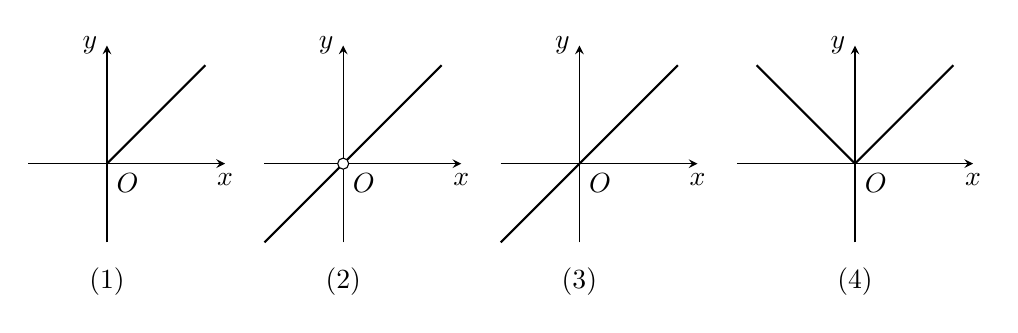
\begin{tikzpicture}[>=stealth]
\begin{scope}
\draw[->](-1,0)--(1.5,0)node[below]{$x$};
\draw[->](0,-1)--(0,1.5)node[left]{$y$};
\node at (0,0)[below right]{$O$};
\draw[thick](0,0)--(1.25,1.25);
\node at (0,-1.5){(1)};

\end{scope}
\begin{scope}[xshift=3cm]
    \draw[->](-1,0)--(1.5,0)node[below]{$x$};
    \draw[->](0,-1)--(0,1.5)node[left]{$y$};
    \node at (0,0)[below right]{$O$};
    \draw[thick](-1,-1)--(1.25,1.25);
    \node at (0,-1.5){(2)};
\draw[fill=white](0,0)circle(2pt);
    \end{scope}
    \begin{scope}[xshift=6cm]
        \draw[->](-1,0)--(1.5,0)node[below]{$x$};
        \draw[->](0,-1)--(0,1.5)node[left]{$y$};
        \node at (0,0)[below right]{$O$};
        \draw[thick](-1,-1)--(1.25,1.25);
        \node at (0,-1.5){(3)};
        
        \end{scope}

\begin{scope}[xshift=9.5cm]
\draw[->](-1.5,0)--(1.5,0)node[below]{$x$};
\draw[->](0,-1)--(0,1.5)node[left]{$y$};
\node at (0,0)[below right]{$O$};
\draw[thick](-1.25,1.25)--(0,0)--(1.25,1.25);
\node at (0,-1.5){(4)};

\end{scope}
\end{tikzpicture}
    \caption{}
\end{figure}

$\because\quad $一个函数由对应法则$f$和定义域$D$唯一确定,

$\therefore\quad $只有当$f$、$D$都相同时,两个解析式才表示同一个函
数。

这四个函数中只有(3)与$y=x$是同一个函数。
\end{solution}

\begin{example}
    乒乓球每个0.5元,买$x$个所用的钱数(元)
\[y=0.5x,\quad x\in\N\]
画出这个函数的图象。
\end{example}

\begin{solution}
    这个函数的定义域是自然数集$\N$, 它的图象由一组
    孤立的点组成(图2.8).
\end{solution}

\begin{example}
    投寄本埠平信,每封信不超过10克的付邮资10分。
超过10克而不超过20克的付邮资20分,以此类推。每封$x\; (0
x\le 30)$
克重的信应付邮资为$y$元:
\[y=\begin{cases}
    10,& x\in(0,10]\\
    20,& x\in(10,20]\\
    30,& x\in(20,30]\\
\end{cases}\]
画出这个函数的图象。
\end{example}

\begin{solution}    
    这个函数的图象由3条线段组成(图2.9).
\begin{figure}[htp]
    \centering
\begin{minipage}{.45\textwidth}
\begin{tikzpicture}[>=stealth]
\draw[->](-.5,0)--(5,0)node[below]{$x$};
\node at (0,0)[below left]{$O$};
\draw[->](0,-1)--(0,3)node[left]{$y$};
\foreach \x in{1,2,3,4}
{
    \draw(\x,0)--(\x,.1);
}
\foreach \x in{1,2}
{
    \draw(0,\x)--(.1,\x);
}

\foreach \x in{1,2,3,4,5}
{
    \draw[fill](\x, 0.5*\x)circle(2pt);
}
\node at (0,1)[left]{1};
\node at (1,0)[below]{1};


\end{tikzpicture}
\caption{}
\end{minipage}
\hfill
\begin{minipage}{.45\textwidth}
    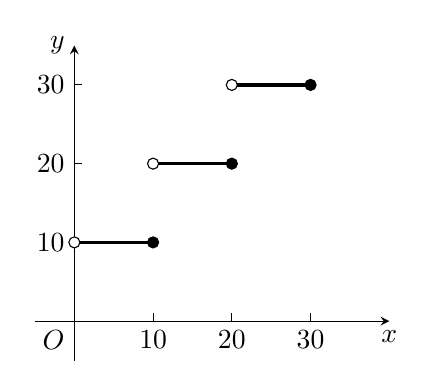
\begin{tikzpicture}[>=stealth]
        \draw[->](-.5,0)--(4,0)node[below]{$x$};
\node at (0,0)[below left]{$O$};
\draw[->](0,-.5)--(0,3.5)node[left]{$y$};
\foreach \x in{1,2,3}
{
    \draw(\x,0)node[below]{\x0}--(\x,.1);
    \draw(0,\x)node[left]{\x0}--(.1,\x);
}
\foreach \x in {1,2,3}
{
    \draw[very thick](\x-1,\x)--(\x,\x);
    \draw[fill](\x, \x)circle(2pt);
    \draw[fill=white](\x-1, \x)circle(2pt);
}



    \end{tikzpicture}
    \caption{}
    \end{minipage}
\end{figure}
\end{solution}

\begin{note}
\begin{enumerate}
    \item  函数的图象通常是一条或几条光滑的曲线,但有
    的函数的图象也可以由一些孤立的点或线段组成(如图2.8, 
    2.9).
    \item 一个函数,对于自变量的不同取值范围,有着不
    同的对应法则,这样的函数(如例2.8中的函数)称为\textbf{分段函
    数}。
\end{enumerate}
\end{note}

\section*{习题三}
\begin{center}
    \bfseries A
\end{center}

\begin{enumerate}
\item \begin{enumerate}[(1)]
    \item 某人有50元去买工具书。已知每本6元,写出所剩
    钱数$y$(元)与买下的书的本数 $x\; (x\ge 0)$
    之间的函数关系
    式。(注意:据实际问题应写出函数的定义域)
    \item 长方形的面积是60${\rm cm}^2$. 写出它的长$y$(cm)与它的宽$x$(cm)的函数关系式。
    \item  在一段笔直的河道上,有相距$d$公里的两城$A$、$B$. 
    过$B$城且垂直河道方向上距$B$城$\ell$公里处有一个工厂$C$. 
    从$A$城运货到工厂,先从水路运到$M$处,然后从$M$走陆
    路到$C$. 假设一吨货物每公里水路运费为$a$元,陆路运费
    为$b$元。求每吨总运费与$MB$之间的函数关系式。
    \item 如图,灌溉渠的横断面是等腰梯形,底宽2米。
    边坡的倾角为$45^{\circ}$, 水深$h$米。求横断面中有水面积$A$米$^2$
    与水深$h$米的函数关系式。
\end{enumerate} 

\begin{center}
\begin{tikzpicture}[>=stealth, decoration=brace]
\begin{scope}
\coordinate (A) at (-3,0);
\coordinate (M) at (0,0);
\coordinate (B) at (2,0);
\coordinate (C) at (2,2);
\draw[very thick,->](A)node[below]{$A$}--(M)node[below]{$M$};
\draw(M)--(B);
\draw[dashed](B)node[below]{$B$}--node[right]{$\ell$}(C);
\draw[very thick,->](M)--(C)node[above]{$C$};
\draw[decorate, decoration={brace, raise=2}](B)--node[below=3pt]{$x$}(M);
\draw[decorate, decoration={brace, raise=2}](A)--node[above=3pt]{$d-x$}(M);
\node at (0,-1){第(3)题};
\end{scope}
\begin{scope}[xshift=5.5cm]
\draw[<->](-1,-.25)--node[fill=white]{2米}(1,-.25);
\fill[cyan!40!white](-2,1)--(-1,0)--(1,0)--(2,1)--cycle;

\node at (0,-1){第(4)题};
\draw[thick](-2.5,1.5)--(-1,0)--(1,0)--(2.5,1.5);
\draw(3,0)--(1,0);
\draw(2,1)--(3,1);
\draw(-1,0)--(-1,-.5);
\draw(1,0)--(1,-.5);
\draw[<->](2.75,0)--node[fill=white]{$h$米}(2.75,1);
\node at (1.8,.25){$45^{\circ}$};
\draw (1.5,0) arc (0:45:.5);
\end{scope}
\end{tikzpicture}
\end{center}

\item 求下列函数的定义域:
\begin{multicols}{2}
\begin{enumerate}[(1)]
    \item $f(x)=3x^{2}-5x+\sqrt{5}$;
    \item $ f\left(x\right)=\frac{1}{2x-3}$;
    \item $ f\left(x\right)=\frac{x+3}{\left(x-2\right)\left(x+3\right)}$;
\item     $f(x) =\frac{\sqrt{x+2}}{x+1}$;
\item     $f(x) =\sqrt{2x-1}+\sqrt{1-2x}$;
\item    $ f\left(x\right)= \sqrt{x-1}\cdot\sqrt{x+1}$ ;
\item     $f\left(x\right)=\sqrt{x^{2}-1}+\sqrt{-|x-3|}$.
\end{enumerate}
\end{multicols}

\item 选择题:下面(\quad)中的一组函数
$f(x)$与$g(x)$是同一个函数:
\begin{enumerate}[(A)]
    \item $f(x)=x^2,\; x\in\R;\qquad g(x)=x^2,\; x\in\R^+$
    \item $f(x)=x+1;\qquad g(x)=\frac{x^2-1}{x-1}$
    \item $f(x)=\sqrt{\frac{x+1}{x-1}};\qquad g(x)=\frac{\sqrt{x+1}}{\sqrt{x-1}}$
    \item $f(x)=\sqrt{x^2};\qquad g(x)=|x|$
\end{enumerate}
\item 海拔高度与气温的对照表为
\begin{center}
    \begin{tabular}{c|cccccc}
\hline
        高度$h$(米)& 0 & 500 & 1000 & 2000 & 3000& 5000\\
\hline
气温$t$ (\oc) &15.00 &11.75& 8.50& 2.00& $-4.50$& $-17.50$ \\
\hline        
    \end{tabular}
\end{center}
\begin{enumerate}[(1)]
    \item 将相应的$(h,t)$作为坐标,在直角坐标系中作
    出各点,由此能看出$t$与$h$满足什么样的函数关系式?
    \item 试求出$t$与$h$的函数关系式。
    \item 能否知道你求出的关系式是否正确?
\end{enumerate}

\item 画出下列函数的图象:
\begin{multicols}{2}
    \begin{enumerate}[(1)]
    \item 正比例函数$y=-2x$;
    \item 反比例函数$y=\frac{8}{x}$;
    \item 反比例函数$y=-\frac{4}{x}$;
    \item 一次函数$y=-4x+5$;
    \item $y=|x|$.
\end{enumerate}
\end{multicols}

\item 画出下列函数的图象:
\begin{multicols}{2}
\begin{enumerate}[(1)]
    \item $y=3x-5,\; x\in(-2,4]$;
    \item $y=2|x|+1,\; x\in\Z,\;\text{且}|x|\le 2$;
    \item $y=|x|-1,\; x\in\R$;
    \item $y=\begin{cases}
        1,& x\in (0,+\infty)\\
        0,&x=0\\
        -1,&x\in(-\infty,0).
    \end{cases}$
\end{enumerate}
\end{multicols}

\item 在国内投寄外埠平信,每封信不超过10克的付邮资20分,
超过10克而不超过20克的付邮资40分,以此类推,写出邮
资(分)与信件重量(不超过40克)的函数关系式,并画出
函数的图象。
\item 画出下列函数的图象:
\begin{multicols}{2}
\begin{enumerate}[(1)]
    \item $y=x^2$;
    \item $y=-\frac{1}{3}x^2$;
    \item $y=x^2-3$;
    \item $y=-\frac{1}{3}x^2+2$;
    \item $y=3(x+2)^2-4$;
    \item $y=-\frac{1}{2}x^2+3x-\frac{5}{2}$.
\end{enumerate}
\end{multicols}
\end{enumerate}


\subsection{函数图象的几何变换}
函数图象的几何变换是研究函数的一种重要工具。

\begin{thm}{问1}
设函数$y=\frac{1}{3}x^2$的图象是$C_1$(图2.10). 若以$x$轴
为对称轴作$C_1$的对称图形得到$C_2$, 你能求出以$C_2$为图象的函
数的解析式吗?
\end{thm}

\begin{figure}[htp]
    \centering
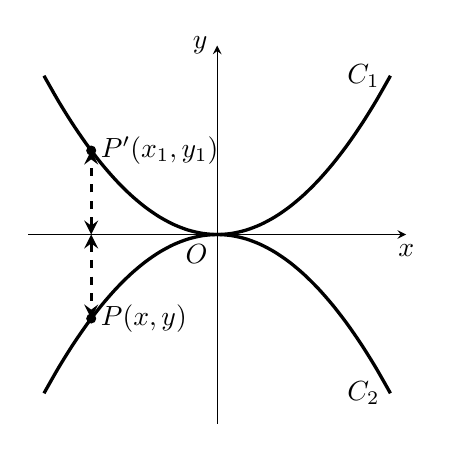
\begin{tikzpicture}[>=stealth, scale=.8]
  \draw[->](-3,0)--(3,0)node[below]{$x$};
\draw[->](0,-3)--(0,3)node[left]{$y$};
\draw[domain=-2.75:2.75, smooth, very thick]plot(\x, 1/3*\x*\x)node[left]{$C_1$};
\draw[domain=-2.75:2.75, smooth, very thick]plot(\x, -1/3*\x*\x)node[left]{$C_2$};  
\node at (0,0)[below left]{$O$};
\node at (-2,4/3)[right]{$P'(x_1,y_1)$};
\node at (-2,-4/3)[right]{$P(x,y)$};
\draw[dashed,<->, very thick](-2,0)--(-2,4/3);
\draw[dashed,<->, very thick](-2,0)--(-2,-4/3);
\draw[fill](-2,4/3) circle (2pt);
\draw[fill](-2,-4/3) circle (2pt);

\end{tikzpicture}
    \caption{}
\end{figure}

\begin{analyze}
    因为两个图象$C_1$与$C_2$关于$x$轴对称,因此它们的
对应点的坐标之间一定具有某种关系,揭示了这种关系,借
助$C_1$的解析式就能得到$C_2$的解析式。
\end{analyze}

设$P(x,y)$是$C_2$上的任
意点,它关于$x$轴的对称点为
$P'(x_1,y_1)$,则
\begin{equation}
\begin{cases}
    x=x_1\\
    y=-y_1
\end{cases}\Longrightarrow \begin{cases}
    x_1=x\\ y_1=-y
\end{cases}
\end{equation}
$\because\quad P'(x_1,y_1)$在$C_1$上,把关系式(2.1)代入$C_1$的解析式$y_1=\frac{1}{3}x^2_1$,得
\[-y=\frac{1}{3}x^2 \Longrightarrow y=-\frac{1}{3}x^2\]
这就是$C_2$上的任一点
$P(x,y)$
满足的关系,也就是以$C_2$为图
象的函数的解析式。

一般地,若函数$y=f(x)$的图象为$C_1$, 作$C_1$关于$x$轴的
对称图象$C_2$, 这种几何变换称为\textbf{函数图象关于$x$轴的对称变
换},此时$C_2$的解析式为$y=-f(x)$(图2.11).

\begin{figure}[htp]
    \centering
\begin{minipage}{.45\textwidth}
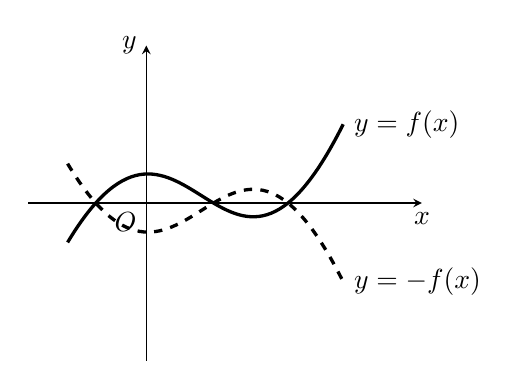
\begin{tikzpicture}[scale=.5, >=stealth]
\draw[->](-3,0)--(7,0)node[below]{$x$};
\draw[->](0,-4)--(0,4)node[left]{$y$};
\node  [below left]{$O$};
\draw[very thick](-2,-1)..controls (1,4) and (2,-4) ..(5,2)node[right]{$y=f(x)$};
\draw[very thick,dashed](-2,1)..controls (1,-4) and (2,4) ..(5,-2)node[right]{$y=-f(x)$};

\end{tikzpicture}
    \caption{}
\end{minipage}
    \hfill
\begin{minipage}{.45\textwidth}
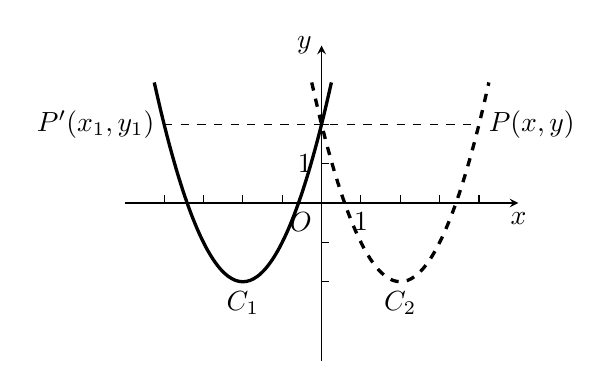
\begin{tikzpicture}[scale=.5, >=stealth]
    \draw[->](-5,0)--(5,0)node[below]{$x$};
    \draw[->](0,-4)--(0,4)node[left]{$y$};
    \node [below left]{$O$};
\draw[domain=-4.25:.25, smooth, very thick]plot(\x, \x*\x+4*\x+2);
\draw[domain=-.25:4.25, smooth, very thick, dashed]plot(\x, \x*\x-4*\x+2);
\draw[dashed](-4,2)node[left]{$P'(x_1,y_1)$}--(4,2)node[right]{$P(x,y)$};
\foreach \x in {-4,-3,...,4}
{
    \draw(\x,0)--(\x,.2);
}
\node at (1,0)[below]{1};
\node at (0,1)[left]{1};

\foreach \x in {-2,-1,...,2}
{
    \draw(0,\x)--(.2,\x);
}
\node at (-2,-2)[below]{$C_1$};
\node at (2,-2)[below]{$C_2$};


\end{tikzpicture}
    \caption{}
\end{minipage}
\end{figure}

\begin{thm}{问2}
     设函数
$y=(x+2)^2-2$
的图象是$C_1$(图2.12). 若
以$y$轴为对称轴作$C_1$的对称图形得到$C_2$, 你能求以$C_2$为图象
的函数的解析式吗?
\end{thm}

类似上面的分析,设$P(x,y)$
为$C_2$上的任意点,它在
$C_1$上的关于$y$轴的对称点为
$P'(x_1,y_1)$,则
\begin{equation}
    \begin{cases}
        x=-x_1\\
        y=y_1
    \end{cases}\Longrightarrow \begin{cases}
        x_1=-x\\ y_1=y
    \end{cases}
\end{equation}
把关系式(2.2)代入$C_1$的解析式
$y_1=(x_1+2)^2-2$,得
$y=(-x+2)^2-2$, 这就是$C_2$上的任一点$P(x,y)$满足的关系,
也就是以$C_2$为图象的函数的解析式。

一般地,若函数$y=f(x)$的图象为$C_1$,作$C_1$关于$y$轴的对称图象
$C_2$,这种几何变换称为\textbf{函数图象关于$y$轴的对称变
换},此时$C_2$的解析式为
$y=f(-x)$(图2.12).

\begin{thm}{问3}
设函数$y=\frac{1}{3}x^2$的图象为$C_1$
,若把$C_1$沿$y$轴向上平移2个单位得到$C_2$(图2.13). 你能求出以
$C_2$为图象的函数的解析式吗?
\end{thm}

类似上面的分析,设$P(x,y)$为$C_2$上的任意点,它在
$C_1$上的对应点为$P'(x_1,y_1)$,则
\begin{equation}
    \begin{cases}
        x=x_1\\y=y_1+2
    \end{cases}\Longrightarrow \begin{cases}
        x_1=x\\y_1=y-2
    \end{cases}
\end{equation}
把(2.3)代入$C_1$的解析式
$y_1=-\frac{1}{3}x_1^2$,得
\[y-2=\frac{1}{3}x^2\Longrightarrow y=\frac{1}{3}x^2+2\]
这是$C_2$上的任意点满足的关系,也就是以
$C_2$为图象的函数的
解析式。

一般地,若把函数
$y=f(x)$
的图象$C_1$沿$y$轴方向平移
$|m|\; (m\in\R)$个单位得到
$C_2$(当$m>0$
时向上移动,当
$m<0$时向下移动),这种几何变换称为\textbf{函数图象的纵向平移变换}。此
时$C_2$的解析式为
\[y=f(x)+m\]

\begin{figure}[htp]
    \centering
\begin{minipage}{.45\textwidth}
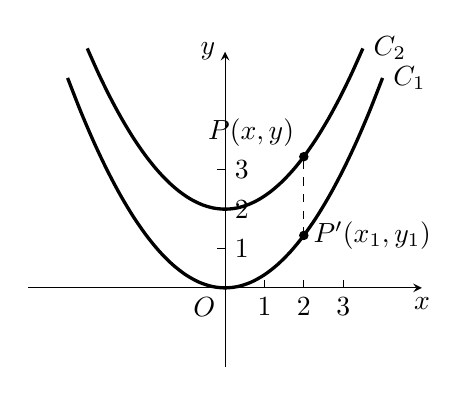
\begin{tikzpicture}[scale=.5, >=stealth]
\draw[->](-5,0)--(5,0)node[below]{$x$};
\draw[->](0,-2)--(0,6)node[left]{$y$};
\node  [below left]{$O$};
\draw[domain=-4:4, smooth, very thick]plot(\x, 1/3*\x*\x)node[right]{$C_1$};
\draw[domain=-3.5:3.5, smooth, very thick]plot(\x, 1/3*\x*\x+2)node[right]{$C_2$};
\foreach \x in{1,2,3}
{
    \draw(\x,0)node[below]{\x}--(\x,.2);
    \draw(0,\x)node[right]{\x}--(-.2,\x);
}

\draw[dashed](2,1.333)node[right]{$P'(x_1,y_1)$}--(2,3.333)node[above left]{$P(x,y)$};
\draw[fill](2,1.333) circle(3pt);
\draw[fill](2,1.333+2) circle(3pt);



\end{tikzpicture}
    \caption{}
\end{minipage}
    \hfill
\begin{minipage}{.45\textwidth}
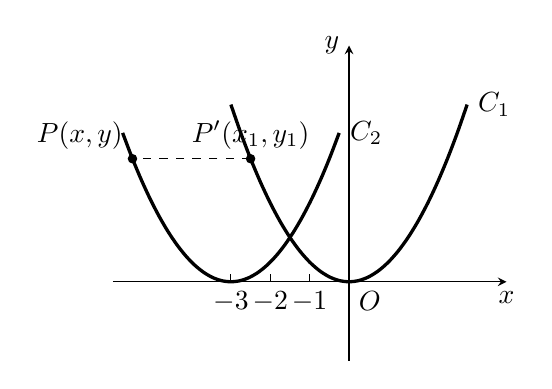
\begin{tikzpicture}[scale=.5, >=stealth]
    \draw[->](-6,0)--(4,0)node[below]{$x$};
    \draw[->](0,-2)--(0,6)node[left]{$y$};
    \node [below right]{$O$};
\draw[domain=-3:3, smooth, very thick]plot(\x, 0.5*\x*\x)node[right]{$C_1$};
\draw[domain=-5.75:-.25, smooth, very thick]plot(\x, 0.5*\x*\x+3*\x+4.5)node[right]{$C_2$};
\foreach \x in {-2,-3,-1}
{
    \draw(\x,0)node[below]{$\x$}--(\x,.2);
}
\draw[dashed](-2.5,3.125)node[above]{$P'(x_1,y_1)$}--(-5.5,3.125)node[above left]{$P(x,y)$};
\draw[fill](-5.5,3.125) circle(3pt);
\draw[fill](-2.5,3.125) circle(3pt);

\end{tikzpicture}
    \caption{}
\end{minipage}
\end{figure}

\begin{thm}{问4}
    设函数$y=\frac{1}{2}x^2$的图象为
    $C_1$,若把$C_1$沿$x$轴向左平移3个单位得到$C_2$(图2.14). 试求出以$C_2$为图象的函数的解析式。
\end{thm}

设$C_2$上的任意点$P(x,y)$,在
$C_1$上的对应点为$P'(x_1,y_1)$,则
\begin{equation}
    \begin{cases}
        x=x_1-3\\y=y_1
    \end{cases}\Longrightarrow \begin{cases}
        x_1=x+3\\y_1=y
    \end{cases}
\end{equation}
把关系(2.4)代入$C_1$的解析式$y_1=\frac{1}{2}x^2_1$,得
\[y=\frac{1}{2}(x+3)^2\]
这就是$C_2$上的任意点$P(x,y)$满足的关系,也就是以$C_2$为
图象的函数的解析式。

一般地,若把函数$y=f(x)$
的图象$C_1$沿$x$轴方向平移
$|m|\; (m\in\R)$个单位得到
$C_2$(当$m>0$时向左移动,当$m<0$时向
右移动),这种几何变换称为\textbf{函数图象的横向平移变换}。此时
得到的$C_2$的解析式为
\[y=f(x+m)\]

\begin{example}
    下列各题中,函数
$f_2(x)$
的图象可由
$f_1(x)$
的图象经过怎样的几何变换得到:
\begin{enumerate}[(1)]
    \item $f_1(x)=3x^2,\quad f_2(x)=-3x^2$;
    \item $f_1(x)=-\frac{1}{2}x^2,\quad f_2(x)=-\frac{1}{2}x^2-3$;
    \item $f_1(x)=\frac{1}{2}x^2,\quad f_2(x)=\frac{1}{2}(x-4)^2$;
    \item $f_1(x)=\frac{1}{2}x^2,\quad f_2(x)=\frac{1}{2}(x+5)^2+3$.
\end{enumerate}
\end{example}

\begin{solution}
\begin{enumerate}[(1)]
    \item 把$f_1(x)$
    的图象作关于$x$轴的对称变换。
    \item 把    $f_1(x)$
    的图象沿
    $y$
    轴向下平移3个单位。
    \item 把    $f_1(x)$
    的图象沿$x$轴向右平移4个单位。
    \item 把    $f_1(x)$
    的图象沿$x$轴向左平移5个单位,再沿$y$轴向
    上平移3个单位。
\end{enumerate}
\end{solution}

\begin{thm}{问5}
    下列各题中的两个函数、图象间有什么关系:
\begin{enumerate}[(1)]
    \item $y=f(x)$与$y=|f(x)|$;
    \item  $y=f(x)$与$y=f(|x|)$.
\end{enumerate}
\end{thm}

\begin{analyze}
    从每个函数的$x$、$y$之间的对应关系进行分析.
\begin{enumerate}[(1)]
    \item 对于相同的$x$值,由
\[y=|f(x)|=\begin{cases}
    f(x), f(x)\ge 0\\
    -f(x), f(x)<0
\end{cases}\]
    知道,当$f(x)\ge 0$时,两函数值相同;当
    $f(x)<0$    时,两函    数值相反。所以,把函数
    $y=f(x)$
    的图象做如下处理:$x$轴
    上方的部分保持不变,$x$轴下方的部分对称到$x$轴上方去,
    这样得到的就是
    $y=|f(x)|$
    的图象(图2.15).

\begin{figure}[htp]
    \centering
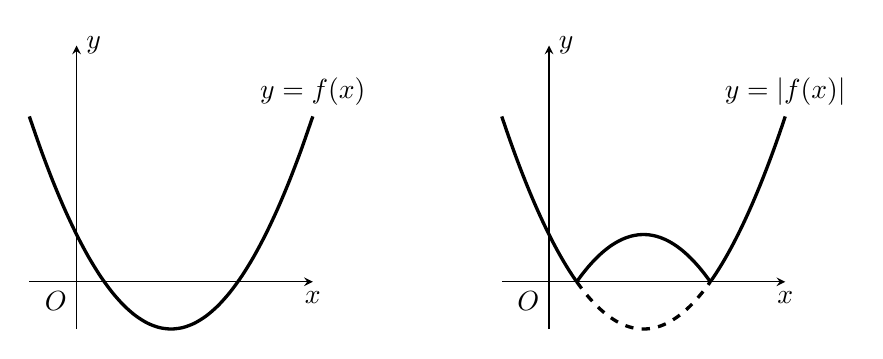
\begin{tikzpicture}[>=stealth, scale=.6]
\begin{scope}
\draw[->](-1,0)--(5,0)node[below]{$x$};
\draw[->](0,-1)--(0,5)node[right]{$y$};
\node [below left]{$O$};
\draw[domain=-1:5, smooth, very thick]plot(\x, .5*\x*\x-2*\x+1)node[above]{$y=f(x)$};
\end{scope}
\begin{scope}[xshift=10cm]
    \draw[->](-1,0)--(5,0)node[below]{$x$};
\draw[->](0,-1)--(0,5)node[right]{$y$};
\node [below left]{$O$};
\draw[domain=-1:2-1.414, smooth, very thick]plot(\x, .5*\x*\x-2*\x+1);
\draw[domain=2+1.414:5, smooth, very thick]plot(\x, .5*\x*\x-2*\x+1)node[above]{$y=|f(x)|$};
\draw[domain=2-1.414:2+1.414, smooth, very thick]plot(\x, -.5*\x*\x+2*\x-1);
\draw[domain=2-1.414:2+1.414, smooth, very thick, dashed]plot(\x, .5*\x*\x-2*\x+1);
\end{scope}
\end{tikzpicture}
    \caption{}
\end{figure}    

 \item 对于函数
    $y=f(|x|)$    来说,当自变量$x$取互为相
    反的数时,函数值总相等,即$f(|x|)=f(|-x|)$
    ,所以函数$y=f(|x|)$
    的图象总是关于$y$轴的对称图形。又,当
    $x\ge 0$    时,    $y=f(x)$
    与 $y=f(|x|)$
    完全相同,因此,把
    $y=f(x)$
    的图象做如下处理,就可得到
    $y=f(|x|)$
    的图象:保留函数
    $y=f(x)$
    图象在$y$轴及$y$轴右侧的部分,去掉在$y$轴左侧的部分,
    然后再把$y$轴右侧的图象对称到$y$轴左侧去(图2.16).

\begin{figure}[htp]
    \centering
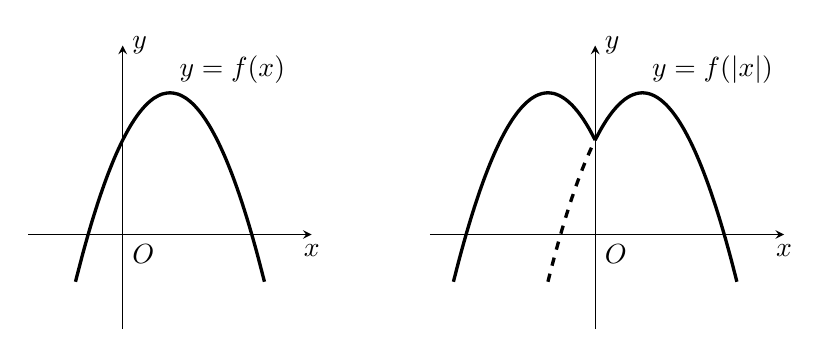
\begin{tikzpicture}[>=stealth, scale=.6]
\begin{scope}
\draw[->](-2,0)--(4,0)node[below]{$x$};
\draw[->](0,-2)--(0,4)node[right]{$y$};
\node [below right]{$O$};
\draw[domain=-1:3, smooth, very thick]plot(\x, -\x*\x+2*\x+2);
\node at (1,3)[above right]{$y=f(x)$};
\end{scope}
\begin{scope}[xshift=10cm]
    \draw[->](-3.5,0)--(4,0)node[below]{$x$};
    \draw[->](0,-2)--(0,4)node[right]{$y$};

\node [below right]{$O$};
\draw[domain=0:3, smooth, very thick]plot(\x, -\x*\x+2*\x+2);
\draw[domain=-1:0, smooth, very thick, dashed]plot(\x, -\x*\x+2*\x+2);
\draw[domain=-3:0, smooth, very thick]plot(\x, -\x*\x-2*\x+2);
\node at (1,3)[above right]{$y=f(|x|)$};
\end{scope}
\end{tikzpicture}
    \caption{}
\end{figure}    
\end{enumerate}
\end{analyze}

\section*{习题四}
\begin{center}
    \bfseries A
\end{center}

下列各题中,函数
$f_2(x)$的图象可由
$f_1(x)$的图象经过怎
样的几何变换得到:
\begin{enumerate}[(1)]
    \item $f_1(x)=-7x^2,\qquad f_2(x)=7x^2$;
    \item $f_{1}(x)=x+3,\qquad f_{2}(x)=-x+3$;
    \item $f_{1}(x)=2(x+2)^{2},\qquad f_{2}(x)=2(x-2)^{2}$;
    \item $f_{1}(x)=-\frac{1}{2}(x+3)^{2},\qquad f_{2}(x)=-\frac{1}{2}(x+3)^{2}-4$;
    \item $f_{1}(x)=-\frac{1}{3}x^{2},\qquad f_{2}(x)=-\frac{1}{3}(x+2)^{2}-5$;
    \item $f_{1}(x)=\frac{1}{x},\qquad f_{2}(x)=\frac{1}{x+3}$;
    \item $f_{1}(x)=2x+1,\qquad f_{2}(x)=2(x-5)+1$;
    \item $ f_{1}(x),\qquad f_{2}(x)=f_{1}(x+2)+6$.
\end{enumerate}

\begin{center}
    \bfseries B
\end{center}
\begin{enumerate}[(1)]\setcounter{enumi}{8}
    \item $f_{1}(x),\qquad f_{2}(x)=-f_{1}(x-1)+3$;
    \item $f_{1}(x)=(x-1)^{2}-3,\qquad f_{2}(x)=|(x-1)^{2}-3|$;
    \item $f_{1}(x)=(x-1)^{2}-3,\qquad f_{2}(x)=(| x|-1)^{2}-3$.
\end{enumerate}

\section{函数的单调性}
图2.17与图2.18分别在相应的区间上给出了两组函数,
这两组函数之间性质上的主要区别是什么?
\begin{figure}[htp]
    \centering
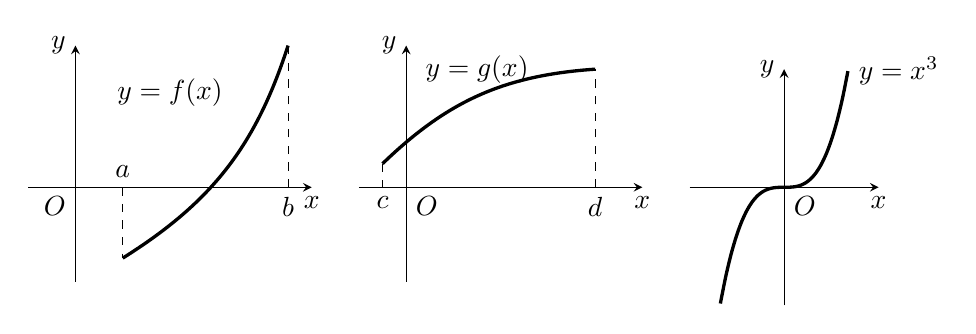
\begin{tikzpicture}[>=stealth, scale=.6]
\begin{scope}
\draw[->](-1,0)--(5,0)node[below]{$x$};
\draw[->](0,-2)--(0,3)node[left]{$y$};
\node[below left]{$O$};

\draw[dashed](1,0)node[above]{$a$}--(1,-1.5);
\draw[dashed](4.5,0)node[below]{$b$}--(4.5,3);
\draw[very thick](1,-1.5)to [bend right=20](4.5,3);

\node at (2,2){$y=f(x)$};
\end{scope}
\begin{scope}[xshift=7cm]
    \draw[->](-1,0)--(5,0)node[below]{$x$};
    \draw[->](0,-2)--(0,3)node[left]{$y$};
\node[below right]{$O$};
\draw[dashed](-.5,.5)--(-.5,0)node[below]{$c$};
\draw[dashed](4,0)node[below]{$d$}--(4,2.5);
\draw[very thick](-.5,.5)to [bend left=20](4,2.5);
\node at (1.5,2.5){$y=g(x)$};

\end{scope}
\begin{scope}[xshift=15cm]
    \draw[->](-2,0)--(2,0)node[below]{$x$};
    \draw[->](0,-2.5)--(0,2.5)node[left]{$y$};
\node[below right]{$O$};
\draw[domain=-1.35:1.35, smooth, very thick]plot(\x, \x^3)node[right]{$y=x^3$};

\end{scope}
\end{tikzpicture}
    \caption{}
\end{figure}

\begin{figure}[htp]
    \centering
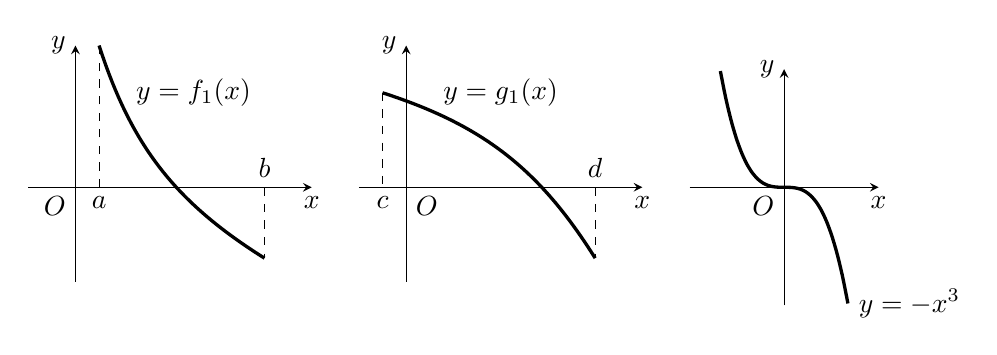
\begin{tikzpicture}[>=stealth, scale=.6]
\begin{scope}
\draw[->](-1,0)--(5,0)node[below]{$x$};
\draw[->](0,-2)--(0,3)node[left]{$y$};
\node[below left]{$O$};

\draw[dashed](4,0)node[above]{$b$}--(4,-1.5);
\draw[dashed](.5,0)node[below]{$a$}--(.5,3);
\draw[very thick](4,-1.5)to [bend left=20](.5,3);

\node at (2.5,2){$y=f_1(x)$};
\end{scope}
\begin{scope}[xshift=7cm]
    \draw[->](-1,0)--(5,0)node[below]{$x$};
    \draw[->](0,-2)--(0,3)node[left]{$y$};
\node[below right]{$O$};
\draw[dashed](-.5,2)--(-.5,0)node[below]{$c$};
\draw[dashed](4,0)node[above]{$d$}--(4,-1.5);
\draw[very thick](-.5,2)to [bend left=20](4,-1.5);
\node at (2,2){$y=g_1(x)$};

\end{scope}
\begin{scope}[xshift=15cm]
    \draw[->](-2,0)--(2,0)node[below]{$x$};
    \draw[->](0,-2.5)--(0,2.5)node[left]{$y$};
\node[below left]{$O$};
\draw[domain=-1.35:1.35, smooth, very thick]plot(\x, -\x^3)node[right]{$y=-x^3$};

\end{scope}
\end{tikzpicture}
    \caption{}
\end{figure}

不难看出:第一组函数,当$x\in$所给区间时,函数值$y$
随$x$的增加而增大;而第二组函数,当$x\in$所给区间时,函数
值$y$随$x$的增加而减小。

下面我们以定义的形式概括这种差别:

\begin{thm}{定义5}
    已知函数$y=f(x)$, $x\in(a,b)$。
\begin{itemize}
    \item 若在$(a,b)$上任取$x_1<x_2$,都有
\[f(x_1)<f(x_2)\]
称$f(x)$在$(a,b)$上是\textbf{增函数},$(a,b)$称为
$f(x)$的\textbf{增区间};
\item 若在$(a,b)$上任取$x_1<x_2$,都有
\[f(x_1)>f(x_2)\]
称$f(x)$在$(a,b)$上是\textbf{减函数},$(a,b)$称为
$f(x)$
的\textbf{减区间}。
\end{itemize}
\end{thm}

增函数与减函数统称\textbf{单调函数},函数的增区间与减区间
统称函数的\textbf{单调区间}。

\begin{note}
\begin{enumerate}
    \item 函数的单调性都是对相应的区间而言的,离开了相
    应的区间就谈不上单调性。因此,在表述单调性时,必须指
    出相应的区间;
    \item 增(减)函数定义的实质是:在相应的区间上,较大
    的$x$值对应较大(小)的$y$值。
\end{enumerate}
\end{note}

\begin{example}
已知$y=f(x),\; x\in[-5,8]$(图2.19), 说出
$f(x)$
的单调区间。
\begin{figure}[htp]
    \centering
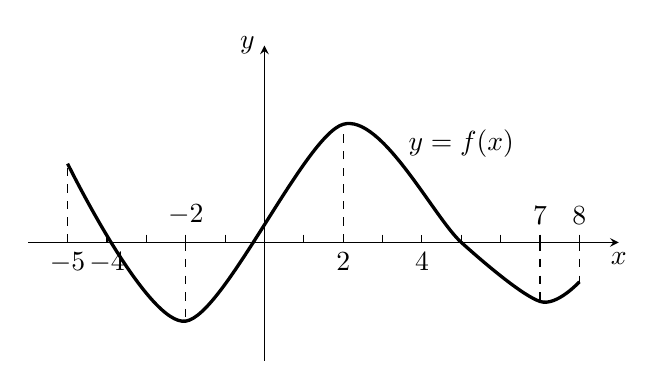
\begin{tikzpicture}[>=stealth, scale=.5]
\draw[->](-6,0)--(9,0)node[below]{$x$};
\draw[->](0,-3)--(0,5)node[left]{$y$};
\draw[dashed](-5,0)--(-5,2);
\draw[dashed](-2,0)--(-2,-2);
\draw[dashed](2,0)--(2,3);
\draw[dashed](7,0)--(7,-1.5);
\draw[dashed](8,0)--(8,-1);
\foreach \x in {-5,-4,2,4}
{
    \draw(\x,0)node[below]{$\x$}--(\x,.2);
}
\foreach \x in {-2,7,8}
{
    \draw(\x,0.2)node[above]{$\x$}--(\x,0);
}
\foreach \x in {1,3,5,6,-1,-3}
{
    \draw(\x,0.2)--(\x,0);
}
\node at (5,2.5){$y=f(x)$};

\draw[very thick] plot[smooth] coordinates{(-5,2) (-2,-2)  (2,3) (5,0) (7,-1.5)(8,-1)};

\end{tikzpicture}
    \caption{}
\end{figure}
\end{example}

\begin{solution}
    增区间有$[-2,2]$和$[7,8]$, 减区间有$[-5,-2]$和
$[2,7]$.

从图象上观察函数的单调性固然形象,但这不够。还必
须学会根据解析式能从数量上分析辨认。后者才是研究函数
单调性的主要途径。
\end{solution}

\begin{example}
    求证函数$f(x)=\frac{1}{x}+1$是$\R$上的增函数。
\end{example}

\begin{proof}
任取$x_1,x_2\in\R$,且$x_1<x_2$,
\[f(x_1)=\frac{1}{2}x_1+1,\qquad f(x_2)=\frac{1}{2}x_2+1\]
\[f(x_1)-f(x_2)=\left(\frac{1}{2}x_1+1\right)-\left(\frac{1}{2}x_2+1\right)=\frac{1}{2}(x_1-x_2)\]

$\because\quad x_1<x_2$

$\therefore\quad x_1-x_2<0,\quad f(x_1)-f(x_2)<0$,即:
\[f(x_1)<f(x_2)\]

$\therefore\quad f(x)$在$\R$上是增函数.
\end{proof}

\begin{example}
    能说反比例函数
$f(x)=\frac{k}{x}\; (k\ne 0)$
在整个定义域
上是单调函数吗?
\end{example}

\begin{figure}[htp]
    \centering
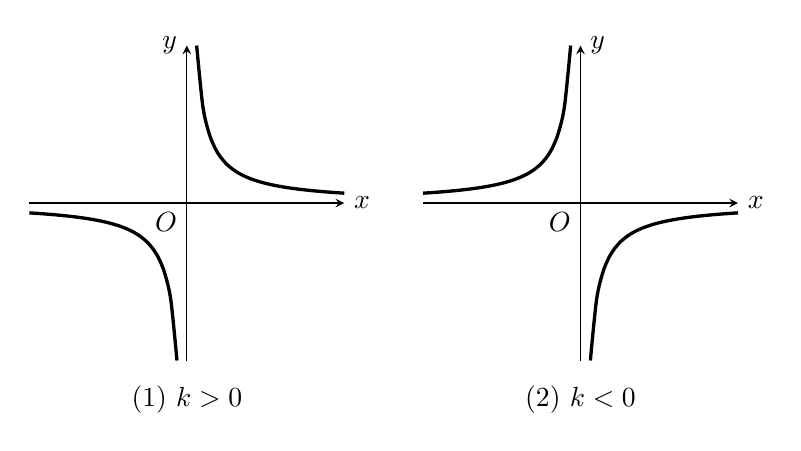
\begin{tikzpicture}[>=stealth, scale=.5]
    \begin{scope}
\draw[->](-4,0)--(4,0)node[right]{$x$};
\draw[->](0,-4)--(0,4)node[left]{$y$};
\node [below left]{$O$};
\draw[domain=-4:-.25, smooth, very thick]plot(\x, 1/\x);
\draw[domain=.25:4, smooth, very thick]plot(\x, 1/\x);
\node at (0,-5){(1) $k>0$};
\end{scope}
\begin{scope}[xshift=10cm]
\draw[->](-4,0)--(4,0)node[right]{$x$};
\draw[->](0,-4)--(0,4)node[right]{$y$};
\node [below left]{$O$};
\draw[domain=-4:-.25, smooth, very thick]plot(\x, -1/\x);
\draw[domain=.25:4, smooth, very thick]plot(\x, -1/\x);
\node at (0,-5){(2) $k<0$};
\end{scope}
\end{tikzpicture}
    \caption{}
\end{figure}

\begin{analyze}
$f(x)$的定义域是$(-\infty,0)\cup (0,+\infty)$.
\begin{enumerate}[(1)]
    \item 当$k>0$时,$f(x)$的图象如图2.20(1)所示。$(-\infty,0)$与$ (0,+\infty)$都是它的减区间,但不能说在整个定义域上
    是减函数。事实上,当取$x_1\in (-\infty,0),\; x_2\in (0,+\infty)$时,$f(x_1)<f(x_2)$,所以,它不是整个定义域上的减函数。
    \item 当$k<0$时,情况类似。(由读者完成)
\end{enumerate}
\end{analyze}

\begin{example}
    求证$f(x)=\frac{k}{x}\; (k>0)$在
$(-\infty,0)$上是减函数。
\end{example}

\begin{proof}
任取$x_1,x_2\in(-\infty,0)$,且$x_1<x_2$(改写成任取$x_1<x_2<0$
也可以),
\[f(x_1)=\frac{k}{x_1},\qquad f(x_2)=\frac{k}{x_2}\]
    \[f(x_1)-f(x_2)=\frac{k}{x_1}-\frac{k}{x_2}=k\cdot \frac{x_1-x_2}{x_1x_2}\]

    由$x_1<x_2<0$, $k>0\Longrightarrow x_1x_2>0$, 
$x_2-x_1>0$,从而
$f(x_1)-f(x_2)>0$,即
\[f(x_1)>f(x_2)\]

$\therefore\quad f(x)$在$(-\infty,0)$上是减函数。
\end{proof}

\begin{example}
求证$f(x)=ax^2+bx+c\; (a<0)$在$\left(-\infty, \frac{-b}{2a}\right]$上是增函数。
\end{example}

\begin{proof}
任取$x_1,x_2\in \left(-\infty, \frac{-b}{2a}\right]$,且$x_1<x_2$
\[f(x_1)=ax_1^2+bx_1+c,\qquad f(x_2)=ax_2^2+bx_2+c\]
\begin{align*}
    f(x_1)-f(x_2)&=a(x_1^2-x_2^2)+b(x_1-x_2)\\
    &=a(x_1-x_2)(x_1+x_2)+b(x_1-x_2)\\
    &=(x_1-x_2)[a(x_1+x_2)+b] \tag{*}
\end{align*}
由$x_1<x_2\Longrightarrow x_1-x_2<0$,而$x_1<\frac{-b}{2a},\; x_2\le \frac{-b}{2a}\Longrightarrow x_1+x_2<\frac{-2b}{2a}=-\frac{b}{a}$

又$\because\quad a<0$

$\therefore\quad a(x_1+x_2)>\left(-\frac{b}{a}\right)a=-b$,从而$a(x_1+x_2)+b>0$

代入(*),可知$f(x_1)-f(x_2)<0$,即
\[f(x_1)<f(x_2)\]
$\therefore\quad f(x)$在$\left(-\infty, \frac{-b}{2a}\right]$上是增函数。
\end{proof}

\begin{example}
$y=x^2-2ax+a^2-1,\; x\in [0,1]$, 试问当$a$取哪些
实数值时,恒有$y>0$.
\end{example}

\begin{analyze}
    这是闭区间$[0,1]$上定义的一个二次函数。欲恒
有$y>0$,只要$y_{\min}>0$($0\le x\le 1$)。为此,考虑抛物线的顶点
位置是重要的。
\end{analyze}

\begin{solution}
    先算出二次函数的顶点$(x_0,y_0)$
\[y=x^2-2ax+a^2-1=(x-a)^2-1\Longrightarrow x_0=a,\; y_0=-1\]

由此,在$[0,1]$上欲使
$y>0$,必须$x_0=a\notin [0,1]$,分两种情况:
\begin{enumerate}[(1)]
    \item 当
$a<0$时(图2.21),这时$y=f(x)$在$[0,1]$上是增函
数,只要
\[y_{\min}=f(0)=a^2-1>0\]
就能保证在$[0,1]$上恒有$y>0$,即
\[\begin{cases}
    a<0\\ a^2-1>0
\end{cases}\Longrightarrow a<-1\]

\begin{figure}[htp]
    \centering
\begin{minipage}{.45\textwidth}
\begin{tikzpicture}[>=stealth]
\draw[->](-2.5,0)--(2.5,0)node[right]{$x$};
\draw[->](0,-1)--(0,4)node[left]{$y$};
\node[below right]{$O$};
\draw[domain=0:1, smooth, very thick]plot(\x, \x*\x+2*\x+.5)node[right]{$y=f(x)$};
\draw[domain=-2:0, smooth, very thick, dashed]plot(\x,  \x*\x+2*\x+.5);
\draw[dashed](1,3.5)--(1,0)node[below]{1};
\node at (-1,-.5)[below]{$(x_0,y_0)$};
\fill(-1,-.5)circle(2pt);

\end{tikzpicture} 
\caption{}
\end{minipage}    \hfill
\begin{minipage}{.45\textwidth}
    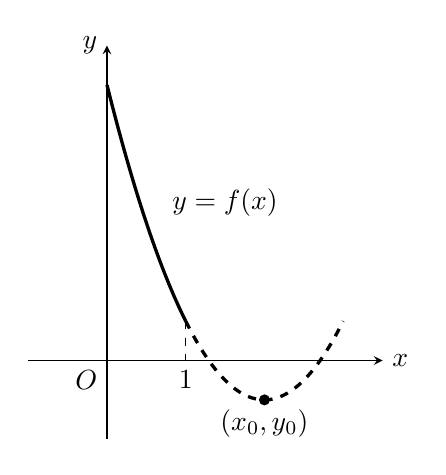
\begin{tikzpicture}[>=stealth]
\draw[->](-1,0)--(3.5,0)node[right]{$x$};
\draw[->](0,-1)--(0,4)node[left]{$y$};
\node[below left]{$O$};
\draw[domain=0:1, smooth, very thick]plot(\x, \x*\x-4*\x+3.5);
\draw[domain=1:3, smooth, very thick, dashed]plot(\x,  \x*\x-4*\x+3.5);
\draw[dashed](1,.5)--(1,0)node[below]{1};
\node at (2,-.5)[below]{$(x_0,y_0)$};
\fill(2,-.5)circle(2pt);
\node at (1.5,2){$y=f(x)$};

    \end{tikzpicture} 
\caption{}
    \end{minipage} 
\end{figure}


\item 当$a>1$时(图2.22),这时
$y=f(x)$
在$[0,1]$上是减函数,只要
\[y_{\min}=f(1)=1^2-2a+a^2-1=a(a-2)>0\]
就能保证在$[0,1]$上恒有
$y>0$, 即
\[\begin{cases}
    a>1\\a(a-2)>0
\end{cases}\Longrightarrow a>2\]

综上所述,当
$a\in (-\infty,-1)\cup (2,+\infty)$
时,恒有$y>0$.
\end{enumerate}
\end{solution}

\begin{thm}{思考题}
    从分析抛物线与$x$轴交点的位置能解出此题吗?若直接
考虑使$y=x^2-2ax+a^2-1>0$
的条件能解此题吗?
\end{thm}

\begin{example}
二次函数$y=f(x)$
的二次项系数为$a\; (a<0)$
,且满足
\begin{equation}
    f(1-x)=f(1+x)  \tag{*}
\end{equation}
\begin{enumerate}[(1)]
\item 这个函数的图象具有什么特征?
\item 写出$f(x)$的单调区间。
\end{enumerate}
\end{example}

\begin{analyze}
    图象的特征由自变量与函数值的对应关系决定。
因此把这种关系分析清楚即可。
\end{analyze}

    \begin{solution}
观察(*)的结构特征可知,当任给一个实数$x$时,
$(1-x)$与$(1+x)$
的值在横轴上对应的点$A$与$B$关于点$(1,0)$
对称(图2.23), 且这两个点对
应的函数值$f(1-x)$与$f(1+x)$
相等。由此,$y=f(x)$
的图象关于直线$x=1$对称,即
$x=1$是图象的对称轴。又因为$a<0$
,所以图象开口向下。但应注意:这里
$y=f(x)$
的条件不足三个,
图象不能唯一确定(图2.23).

$(-\infty,1]$是$f(x)$
的增区间,$[1,+\infty)$是$f(x)$
的减区间。
\end{solution}

\begin{figure}[htp]\centering
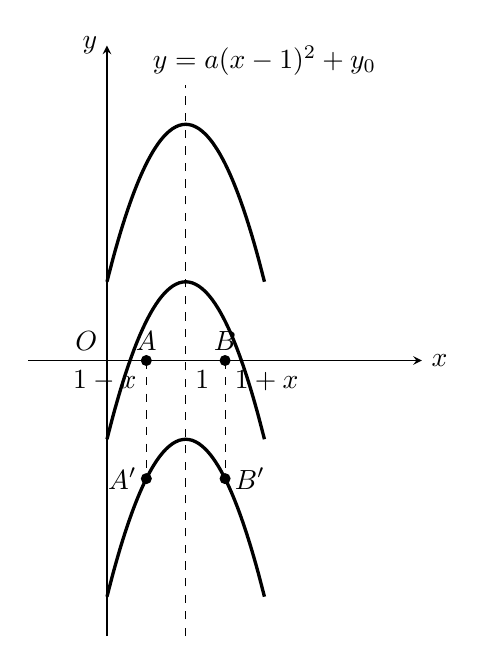
\begin{tikzpicture}[>=stealth]
\draw[->](-1,0)--(4,0)node[right]{$x$};
\draw[->](0,-3.5)--(0,4)node[left]{$y$};
\node [above left]{$O$};
\draw[dashed](1,-3.5)--(1,3.5);
\draw[domain=0:2, smooth, very thick]plot(\x, -2*\x*\x+4*\x+1);
\draw[domain=0:2, smooth, very thick]plot(\x, -2*\x*\x+4*\x-1);
\draw[domain=0:2, smooth, very thick]plot(\x, -2*\x*\x+4*\x-3);
\node at (2,3.5)[above]{$y=a(x-1)^2+y_0$};
\draw[dashed](1.5, 0)node[above]{$B$}--(1.5, .5-2)node[right]{$B'$};
\draw[dashed](.5, 0)node[above]{$A$}--(.5, .5-2)node[left]{$A'$};
\node at (1,0)[below right]{1};
\foreach \x in {.5,1.5}
{
    \fill (\x,0)circle (2pt);
    \fill (\x,-1.5)circle (2pt);
}
\node at (.5,0)[below left]{$1-x$};
\node at (1.5,0)[below right]{$1+x$};
\end{tikzpicture}
    \caption{}
\end{figure}

\section*{习题五}
\begin{center}
\bfseries A
\end{center}

\begin{enumerate}
    \item 说出下列函数的增区间和减区间:
\begin{enumerate}[(1)]
    \item $y=kx\; (k<0),\quad x\in\R$;
    \item $y=ax^2+bx+c\; (a>0),\quad x\in\R$;
    \item $y=1-x^2,\quad x\in\R$;
\end{enumerate}
    \item 证明:
\begin{enumerate}[(1)]
    \item $f(x)=\frac{3}{x}$在$(-\infty,0)$上是减函数;
    \item 当$a<0$时, $f(x)=ax^2\; (x\ge 0)$
    是减函数;
 \item $f(x)=3x^2+12x-5$
    在$(-\infty,-2)$上是减函数;
 \item $f(x)=ax^2+bx+c\; (a<0)$   在$\left(-\infty,\frac{-b}{2a}\right)$上是增函数。
\end{enumerate}
\end{enumerate}


\begin{center}
\bfseries B
\end{center}

\begin{enumerate}\setcounter{enumi}{2}
    \item 对于函数$y=x^3$,
\begin{enumerate}[(1)]
\item 画出它的图象;
\item 写出它的单调区间,并用定义证明之。
\end{enumerate}

\item 函数$f(x)=x^2+ax+3-a$,若
$f(x)$在$[-2,2]$上恒非负,
求实数$a$的取值范围。
\end{enumerate}

\section{函数的奇偶性}
“对称”是大自然的一种美,这种“对称美”经常会反映到
数学中来。让我们看下列各函数(图2.24)有什么共性?
\begin{figure}[htp]
    \centering
\begin{tikzpicture}[>=stealth, scale=.7]
\begin{scope}
\draw[->](-2,0)--(2,0)node[right]{$x$};
\draw[->](0,-1)--(0,3)node[left]{$y$};
\draw[domain=-1.5:1.5, smooth, very thick]plot(\x,\x*\x)node[above]{$y=x^2$};
\node[below left]{$O$};
\node at (0,-1.5){(1)};

\end{scope}
\begin{scope}[xshift=6cm, scale=.6]
\draw[->](-4,0)--(4,0)node[right]{$x$};
\draw[->](0,-1)--(0,5)node[left]{$y$};
\draw[domain=.5:3.5, smooth, very thick]plot(-\x,1/\x^2);
\draw[domain=.5:3.5, smooth, very thick]plot(\x,1/\x^2);
\node[below left]{$O$};
\node at (1,3)[right]{$y=\frac{1}{x^2}$};
\node at (0,-2.5){(2)};
\end{scope}
\begin{scope}[xshift=12cm]
\draw[->](-2.5,0)--(2.5,0)node[right]{$x$};
\draw[->](0,-1)--(0,3)node[left]{$y$};
\draw[domain=0:2.5, smooth, very thick]plot(\x,{\x^(2/3)})node[above]{$y=x^{\tfrac{2}{3}}$};
\draw[domain=0:2.5, smooth, very thick]plot(-\x,{\x^(2/3)});

\node[below left]{$O$};
\node at (0,-1.5){(3)};

    
\end{scope}
\begin{scope}[yshift=-6cm, xshift=1cm]
\draw[->](-3,0)--(3,0)node[right]{$x$};
\draw[->](0,-3)--(0,4.5)node[right]{$y$};
\draw[domain=0:2.2, smooth, very thick]plot(\x,{\x^4-5*\x^2+4})node[above]{$x^4-5x^2+4$};
\foreach \x in{-2,-1,1,2}
{
    \node at (\x,0)[below]{$\x$};
    \node at (0,\x)[left]{$\x$};
    \draw(0,\x)--(.2,\x);
}
\node at (0,-3.5){(4)};
\node [below left]{$O$};

\draw[domain=0:2.2, smooth, very thick]plot(-\x,{\x^4-5*\x^2+4});
\end{scope}
\begin{scope}[yshift=-6cm, xshift=10cm, scale=.8]
\draw[->](-6,0)--(6,0)node[right]{$x$};
\draw[->](0,-3)--(0,3)node[left]{$y$};
\draw[very thick](-5,0)--(-3,-1)--(-1,2);
\draw[very thick](5,0)--(3,-1)--(1,2)node[above right]{$y=f(x)$};
\node at (0,-3.5){(5)};
\foreach \x in {-5,-4,...,5}
{
    \draw(\x,0)--(\x,.2);
}
\foreach \x in {-5,-1,1,5}
{
    \node at (\x,0)[below]{$\x$};
}
\foreach \x in {-3,3}
{
    \node at (\x,.2)[above]{$\x$};
}
\node [below right]{$O$};


\end{scope}
\end{tikzpicture}
    \caption{}
\end{figure}

这些函数的图象都以$y$
轴$C:\; y=f(x)$
为对称轴。即若在函数的图象
$C$上任取一点
$P(x,y)$,必有
$P'(-x,y)\in C$(图2.25).

\begin{figure}[htp]
    \centering
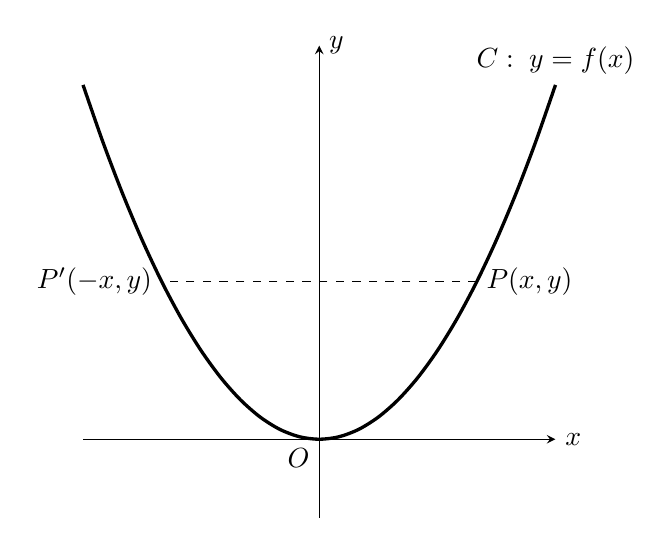
\begin{tikzpicture}[>=stealth]
\draw[->](-3,0)--(3,0)node[right]{$x$};
\draw[->](0,-1)--(0,5)node[right]{$y$};
\draw[domain=-3:3, smooth, very thick]plot(\x, .5*\x*\x)node[above]{$C:\; y=f(x)$};
\node [below left]{$O$};
\draw[dashed](2,2)node[right]{$P(x,y)$}--(-2,2)node[left]{$P'(-x,y)$};
\end{tikzpicture}
    \caption{}
\end{figure}



从图象上可以看出,$x$、$y$
的对应关系上的共性是:自变量的任何两个相反的值,对
应的函数值 都相等,即任取
$x\in D$,都有
$f(-x)=f(x)$.

这类函数的共性是具“对称性”,抓住它有利于:
\begin{enumerate}[(1)]
    \item 方便作图:先作出$x>0$的部分,由对称性可方
    便地画出$x<0$的部分;
    \item 方便函数性质的研究:如
    $f(x)$在$x>0$
    是增函数,那么在$x<0$
    就必是减函数,$f(x)$若在$x>0$上有两个零点,则
    在$x<0$上必存在两个关于原点对称的两个零点,……
\end{enumerate}

正因为如此,这类函数在数学上占有重要地位。下面以
    定义的形式对这类函数做出概括。


\begin{thm}{定义6}
  对于函数$y=f(x),\; x\in D$,若任取
$x\in D$都有
\begin{equation}
    f(-x)=f(x)\tag{*}
\end{equation}
称$f(x)$为\textbf{偶函数}。  
\end{thm}

\begin{note}
\begin{enumerate}
    \item 先看自变量,任取$x\in D$, (*)
都成立,这说明
$f(x)$与$f(-x)$
都有意义,即$x$, $-x$同时属于
$D\Longrightarrow D$
关于原点对称,就是说,定义域$D$关于原点对称是偶函数的 必要条
件;
\item 偶函数定义的实质:任取自变量的两个相反的值,
其对应的函数值都相等;
\item 任取$x\in D$
,(*)都成立。这说明这种性质是$f(x)$
在定义域上的整体性质。
\item 偶函数的图象关于$y$轴成轴对称图形。

这一点证明如下,设函数
$y=f(x)$
是偶函数,则有
$f(-x)=f(x)$
,如图2.25, 在
$f(x)$的图象上任取一点
$P(x,y)$那么$P$点关于$y$轴的对称点是
$P'(-x,y)$,而
$f(-x)=f(x)=y$,说明$P'$点也是函数$f(x)$
图象上的点。这就是说,函数$f(x)$
图象上任意一点关于$y$轴的对称点都在$f(x)$的图象上,所以,偶函数
$y=f(x)$
的图象关于$y$轴成轴对称图形。
\end{enumerate}
\end{note}

\begin{example}
    用定义证明
$f(x)=x^4-5x^2+4$
是偶函数。
\end{example}

\begin{proof}
    首先应明确这里$D=\R$,任取$x\in\R$,
\[\begin{split}
    f(x)&=x^4-5x^2+4\\
    f(-x)&=(-x)^4-5(-x)^2+4=x^4-5x^2+4
\end{split}\]
$\therefore\quad f(-x)=f(x)$

$\therefore\quad f(x)$是偶函数。
\end{proof}

\begin{example}
    下列函数是偶函数吗?
\begin{multicols}{3}
\begin{enumerate}[(1)]
    \item $y=x^2\; (x>0)$;
    \item $y=5$;
    \item $y=|x|$.
\end{enumerate}
\end{multicols}
\end{example}

\begin{analyze}
\begin{enumerate}
    \item 由于定义域关于原点不对称,所以$y=x^2\; (x>0)$不是偶函数;
    \item 对$y=5$而言,$D=\R$,在$\R$上任取两个相反的$x$, 其函数值都是5, 所以$y=5$是偶函数。(由此可知,所有的\textbf{常数函数都是偶函数}!)
    \item $y=f(x)=|x|$,应明确$D=\R$,
    
    $\because\quad $任取:$x\in\R$, $f(x)=|x|$, $f(-x)=|-x|=|x|$,
    $\therefore\quad f(-x)=f(x)$。所以,$y=|x|$是偶函数。
\end{enumerate}
\end{analyze}

\begin{example}
    偶函数$y=f(x)$当$x\ge 0$时是增函数,当$x\le 0$
时,指出其增减性,并证明之。
\end{example}

\begin{solution}
    由于偶函数的图象关于$y$轴对称,当$x\ge 0$时是增函数,则当$x\le 0$
时必是减函数(图2.26是示意图)。证明如下:

任取$x_1,x_2\in(-\infty,0]$,且$x_1<x_2$

$\because\quad f(x)$是偶函数,

$\therefore\quad f(x_1)=f(-x_1),\quad f(x_2)=f(-x_2)$

又$\because\quad x_1<x_2\le 0$,

$\therefore\quad -x_1>-x_2\ge 0$,而$y=f(x)$在$x\ge 0$
上是增函数。

$\therefore\quad f(-x_1)>f(-x_2)$.

由此$f(x_1)-f(x_2)=f(-x_1)-f(-x_2)>0$,即
\[f(x_1)>f(x_2)\]
$\therefore\quad f(x)$在$x\le 0$上是减函数。
\end{solution}

\begin{figure}[htp]
    \centering
\begin{minipage}{.45\textwidth}
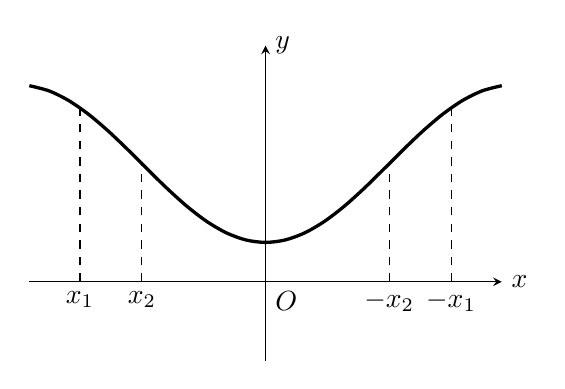
\begin{tikzpicture}[>=stealth]
\draw[->](-3,0)--(3,0)node[right]{$x$};
\draw[->](0,-1)--(0,3)node[right]{$y$};
\node[below right]{$O$};
\draw[domain=-3:3, very thick, smooth]plot(\x, {-cos(\x r)+1.5});
\draw[dashed](-pi/2,0)node[below]{$x_2$}--(-pi/2,1.5);
\draw[dashed](pi/2,0)node[below]{$-x_2$}--(pi/2,1.5);
\draw[dashed](-pi*.75,0)node[below]{$x_1$}--(-pi*.75,.79+1.5);
\draw[dashed](pi*.75,0)node[below]{$-x_1$}--(pi*.75,.79+1.5);
\end{tikzpicture}
\caption{}  
\end{minipage}
\hfill
\begin{minipage}{.45\textwidth}
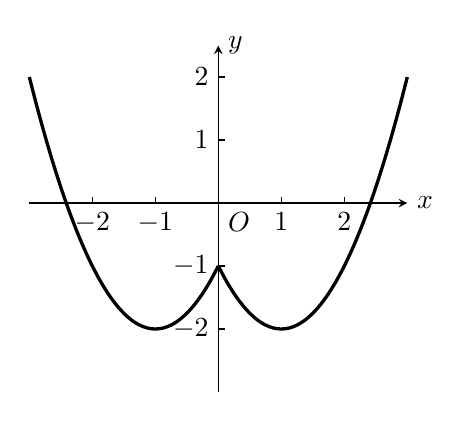
\begin{tikzpicture}[>=stealth, scale=.8]
    \draw[->](-3,0)--(3,0)node[right]{$x$};
\draw[->](0,-3)--(0,2.5)node[right]{$y$};
\node[below right]{$O$};
\draw[domain=0:3, very thick, smooth]plot(\x, \x*\x-2*\x-1);
\draw[domain=0:3, very thick, smooth]plot(-\x, \x*\x-2*\x-1);
\foreach \x in{-2,-1,1,2}
{
    \draw(0,\x)node[left]{$\x$}--(.1,\x);
    \draw(\x,0)node[below]{$\x$}--(\x,.1);
}
\end{tikzpicture}
\caption{}  
\end{minipage}
\end{figure}

\begin{example}
设$f(x)=x^2-2|x|-1\; (-3\le x\le 3)$. 
\begin{enumerate}[(1)]
    \item 画出函数的图象;
    \item 求出方程$f(x)=0$的根;
    \item 指出$f(x)$的单调增区间和单调减区间;
    \item 求出$f(x)$的值域。
\end{enumerate}
\end{example}

\begin{solution}
    应能看出$f(x)$是$[-3,3]$上的偶函数。事实上,$x\in[-3,3]$,
\[f(-x)=(-x)^2-2|-x|-1=x^2-2|x|-1=f(x)\]
$\therefore\quad f(x)$是偶函数。

\begin{enumerate}[(1)]
    \item 可先画出$x\in[-3,3]$上的图象,此时
$f(x)=x^2-2x-1=(x-1)^2-2$。据此,可以作出图象的右半支。再利
用图象关于$y$轴的对称性作出
左半支(图2.27).
\item 当$x\in[0,3]$时, $f(x)=0$有一个根.

令$x^{2}-2x-1=0$, 得$x_1= 1+ \sqrt {2}$, $x_2= 1- \sqrt {2}< 0$(舍)。

$\therefore\quad$一个根是$1+\sqrt2$, 据对称性知另一个根是$-1-\sqrt{2}$。

\item 单调增区间是$[-1,0]$, $[1,3]$;单调减区间是$[-3,-1]$, $[0,1]$。
\item $f(x)$在$[0,3]$上的值域是$[f(1), f(3)]=[-2,2]$, 据对称性知在$[-3,0]$上的值域也是$[-2,2]$.

$\therefore\quad f(x)$
在$D$上的值域是$[-2,2]$.
\end{enumerate}
\end{solution}

\begin{note}
    此例由于利用了偶函数的性质,使作图与性质讨
论都大为简化。
\end{note}

下列函数图象(图2.28)的共性是什么?
\begin{figure}[htp]
    \centering
\begin{tikzpicture}[>=stealth, scale=.9]
\begin{scope}
\draw[->](-1.8,0)--(1.8,0)node[right]{$x$};
\draw[->](0,-2)--(0,2)node[right]{$y$};
\node[below left]{$O$};
\node at (0,-2.5){(a)};
\draw[very thick](-1.5,1.3)--(1.5,-1.3);

\end{scope}
\begin{scope}[xshift=4cm, scale=.5]
\draw[->](-3,0)--(3,0)node[right]{$x$};
\draw[->](0,-4)--(0,4)node[right]{$y$};
\node[below right]{$O$};
\node at (0,-5){(b)};
\draw[domain=-2.5:2.5, smooth, very thick]plot(\x, 0.25*\x*\x*\x)node[above]{$y=\frac{1}{4}x^3$};

\end{scope}
\begin{scope}[xshift=8cm, scale=.5]
    \draw[->](-4,0)--(4,0)node[right]{$x$};
\draw[->](0,-4)--(0,4)node[right]{$y$};
\node[below right]{$O$};
\node at (0,-5){(c)};
\draw[domain=-1.5:1.5, smooth, very thick]plot(\x^3, \x)node[above]{$y=x^{\tfrac{1}{3}}$};

\end{scope}
\begin{scope}[yshift=-5cm, xshift=1.5cm, scale=.5]
    \draw[->](-7,0)--(6,0)node[right]{$x$};
\draw[->](0,-2)--(0,3)node[right]{$y$};
\node[below right]{$O$};
\draw[domain=-6:5, smooth, very thick, samples=100]plot(\x, {sin(\x r)})node[below]{$y=f(x)$};

\node at (0,-2.5){(d)};


\end{scope}
\begin{scope}[yshift=-5cm, xshift=8cm, scale=.5]
    \draw[->](-5,0)--(5,0)node[right]{$x$};
\draw[->](0,-2)--(0,3)node[right]{$y$};
\node[below right]{$O$};
\node at (0,-2.5){(e)};
\draw[very thick](-4,0)--(-3,1.5)--(-1,0);
\draw[very thick](4,0)--(3,-1.5)--(1,0);
\foreach \x in {2,4}
{
    \draw(\x,0)--(\x,.2)node[above]{$\x$};
    \draw(-\x,0)node[below]{$-\x$}--(-\x,.2);
}
\end{scope}
\end{tikzpicture}
    \caption{}
\end{figure}


很明显,函数的图象关于原点成中心对称。可以做如下的概括:

\begin{thm}{定义7}
对于$y=f(x),\; x\in D$,若任取$x\in D$,都有$f(-x)=-f(x)$, 
称$f(x)$为\textbf{奇函数}。
\end{thm}

\begin{note}
\begin{enumerate}
    \item 定义域关于原点对称是奇函数的必要条件;
    \item 奇函数的实质是:定义域中任取自变量的两个相反的值,对应的函数值恰好相反;
    \item 该定义所揭示的函数的性质是定义域上的整体性质。
    \item 奇函数的图象关于原点成中心对称图形(请同学们自己证明)。
\end{enumerate}
\end{note}

\begin{ex}
填空:
\begin{enumerate}[(1)]
    \item $y=x^n\; (n\in\Z)$是偶函数的充要条件是\blank;
    \item $y=x^n\; (n\in\Z)$是奇函数的充要条件是\blank;
    \item $y=ax^2+bx+c\; (a\ne 0)$是偶函数的充要条件是\blank;
    \item $y=ax+b\; (a\ne 0)$是奇函数的充要条件是\blank.
\end{enumerate}
\end{ex}

\begin{thm}{思考题}
    $y=0$是奇函数?还是偶函数?    
\end{thm}

\begin{example}
    奇函数$y=f(x)$在$(-10,0]$上是增函数。那么它在$[0,10)$上是增函数还是减函数?证明你的结论。
\end{example}

\begin{solution}
据图象关于原点成中心对称可知,$f(x)$在$[0,10)$上仍然是增函数,证明如下:

任取$x_1,x_2\in [0,10)$,且$x_1<x_2$ (写成任取$0\le x_1<x_2<10$也可)

$\because\quad y=f(x)$是奇函数,

$\therefore\quad f(x_1)=-f(-x_1),\quad f(x_2)=-f(-x_2)$.

又$\because\quad 0\le x_1<x_2$, $\therefore\quad -x_2<-x_1\le 0$

$\because\quad y=f(x)$在$(-10,0]$上是增函数,

$\therefore\quad f(-x_2)<f(-x_1)$,

从而$f(x_1)-f(x_2)=-f(-x_1)-[-f(-x_2)]=f(-x_2)-f(-x_1)<0$,即
$f(x_1)<f(x_2)$

$\therefore\quad f(x)$在$[0,10)$上是增函数.
\end{solution}

\begin{example}
    求证:在公共定义域上,奇函数与奇函数的积是偶函数。
\end{example}

\begin{proof}
    设$y=f_1(x)$在$D_1$上是奇函数,$y=f_2(x)$在$D_2$上是奇函数。以下证明$F(x)=f_1(x)\cdot f_2(x)$在$D=D_1\cap D_2$上是偶函数。

任取$x\in D$, $F(x)=f_1(x)\cdot f_2(x)$,

$\because\quad D=D_1\cap D_2$

$\therefore\quad x\in D_1$, 且$x\in D_2$,

$\because\quad f_1(x)$是$D_1$上的奇函数

$\therefore\quad f_1(-x)=-f_1(x)$,

$\because\quad f_2(x)$是$D_2$上的奇函数,

$\therefore\quad f_2(-x)=-f_2(x)$。

$\therefore\quad F(-x)=f_1(-x)\cdot f_2(-x)=[-f_1(x)]\cdot [-f_2(x)]
=f_1(x)\cdot f_2(x)=F(x)$。

即:任取$x\in D$,都有$F(-x)=F(x)$。

$\therefore\quad F(x)$在$D$上是偶函数。
\end{proof}

\begin{thm}{思考题}
\begin{enumerate}[(1)]
    \item 这里强调公共定义域是何道理?
    \item 类比此例,你还能猜到哪些结论?能否加以证明?
\end{enumerate}
\end{thm}

\begin{example}
    设$F(x)$是定义在$\R$上的奇函数,且当$x>0$时,$F(x)$的解析式是$f(x)$,求$F(x)$的完整表达式。
\end{example}

\begin{analyze}
    这个题的意义是
\[\text{奇函数}F(x)=\begin{cases}
    f(x), & x>0\\
    ?&x=0\\
    ?&x<0
\end{cases}\]
\end{analyze}

\begin{solution}
任取$x\in (-\infty,0)$,设$P(x,y)$是函数$F(x)$图象上的一个点,由于$F(x)$是奇函数,所以,其图象关于原点对称(图2.29)。由此,$P'(-x,-y)$必然也是图象上的一个点,由于$-x>0$,此时$P'(-x,-y)$必满足 解析式$y=f(x)$. 即
\begin{equation}
    -y=f(-x)\Longrightarrow y=-f(-x)  \tag{*}
\end{equation}

(*)就是点$P(x,y)$的坐标满足的关系式,即$x<0$时$F(x)$的解析式。

当$x=0$时,$f(-0)=-f(0)$,即$f(0)=0$.

$\therefore\quad \text{奇函数}F(x)=\begin{cases}
    f(x), & x>0\\
    0,&x=0\\
    -f(-x),&x<0
\end{cases}$
\end{solution}

\begin{figure}[htp]
    \centering
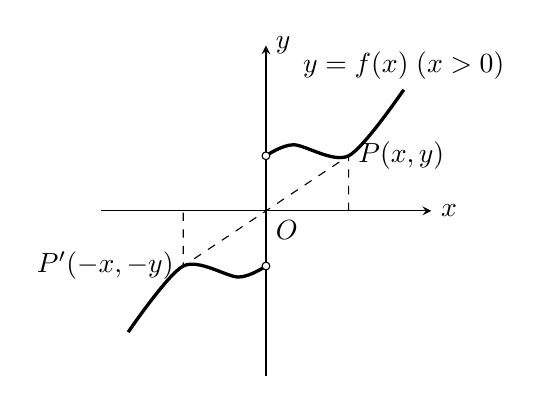
\begin{tikzpicture}[>=stealth, scale=.7]
\draw[->](-3,0)--(3,0)node[right]{$x$};
\draw[->](0,-3)--(0,3)node[right]{$y$};
\draw[very thick]plot[smooth] coordinates{(0,1) (.5,1.2)(1.5,1)(2.5,2.2)};
\draw[very thick]plot[smooth] coordinates{(0,-1) (-.5,-1.2)(-1.5,-1)(-2.5,-2.2)};
\draw[fill=white](0,1)circle(2pt);
\draw[fill=white](0,-1)circle(2pt);
\draw[dashed](1.5,0)--(1.5,1)node[right]{$P(x,y)$}--(-1.5,-1)node[left]{$P'(-x,-y)$}--(-1.5,0);
\node at (2.5,2.2)[above]{$y=f(x)\; (x>0)$};
\node [below right]{$O$};

\end{tikzpicture}
    \caption{}
\end{figure}

\section*{习题六}
\begin{center}
    \bfseries A
\end{center}
\begin{enumerate}
    \item (口答)下列哪些是奇函数?哪些是偶函数?哪些既不是奇函数也不是偶函数(称为非奇非偶函数)?
\begin{multicols}{2}
\begin{enumerate}[(1)]
    \item $y=3x$
    \item $y=-2x+3$
    \item $y=x^2-1$
    \item $y=2x^2+3x-1$
    \item $y=2x^3$
    \item $y=2x^3+1$
    \item $y=x^4-3x^2+1$
    \item $y=x^3+5x$
\end{enumerate}
\end{multicols}
  \item   (口答)同上题:
\begin{multicols}{2}
\begin{enumerate}[(1)]
    \item $y=(x-1)^2+1$
    \item $y=\sqrt{x^2-1}$
    \item $y=x^3+x-1$
    \item $y=x^4-2|x|-5$
    \item $y=|x|+1$
    \item $y=|2x+1|$
\end{enumerate}
\end{multicols}

\item     确定下列函数的奇偶性(“确定”应简述根据):
\begin{multicols}{2}
\begin{enumerate}[(1)]
    \item $f(x)=\frac{1}{x}$
    \item $f(x)=\frac{1}{x+1}$
    \item $f(x)=\frac{7}{x^2+1}$
    \item $f(x)=\frac{x}{x^2-1}$
    \item $f(x)=\frac{1}{x}+\frac{1}{x^3}$
    \item $f(x)=\frac{1}{x^2}+\frac{1}{x^4}-1$
    \item $f(x)=\frac{x^3-x}{x^3+x}$
    \item $f(x)=\frac{|x|}{x}$
\end{enumerate}
\end{multicols}
\end{enumerate}

\begin{center}
    \bfseries B
\end{center}

\begin{enumerate}\setcounter{enumi}{3}
    \item 在公共定义域上,求证:
\begin{enumerate}[(1)]
    \item 偶函数与偶函数的积是偶函数;
    \item 偶函数与奇函数的积是奇函数;
    \item 奇函数与奇函数的积是偶函数。
\end{enumerate}
\item     当$x\in [-b,b]$时,奇函数$y=f(x)$在$[a,b)$上是减函数$(0<a<b)$,那么它在$(-b,-a]$上是增函数还是减函数?证明你的结论。
\item     已知$F(x)$是定义在$\R$上的奇函数,当$x>0$时$F(x)=x(1+x)$,求$F(x)$的完整表达式。
\item    已知$F(x)$是偶函数,当$x\ge 0$时,$F(x)=f(x)$,求$F(x)$的完整表达式。
\item    设$y=f(x)$是定义在R上的任意一个函数,求证:
\begin{enumerate}[(1)]
    \item $F(x)=f(x)+f(-x)$是个偶函数;
    \item $G(x)=f(x)-f(-x)$是个奇函数。
\end{enumerate}
    
\end{enumerate}

\section{反函数}

我们知道:从数集$A$到数集$B$的映射就是定义在$A$上的函数。若已知映射$\map{f}{A}{B}$,其中
\[A=(-\infty,+\infty),\quad B=(-\infty,+\infty),\quad \map{f}{x}{y}=x,\; x\in A\]
很明显,这个映射所确定的函数关系是
\begin{equation}
    y=x^3,\quad x\in A.\tag{1}
\end{equation} 

\begin{thm}{问1}
    这个映射存在逆映射吗?
\end{thm}

\begin{analyze}
    该映射是单射($A$中不同的元,对应着$B$中不同的象),又是满射($B$中任一元,在$A$中都有原象),所以它是从$A$到$B$上的一一映射。从而它存在逆映射:
$\map{f^{-1}}{B}{A}$,其中$\map{f^{-1}}{y}{x}=\sqrt[3]{y},\; y\in B$.
\end{analyze}

\begin{thm}{问2} 
    说出上述逆映射所确定的函数关系?   
\end{thm}

\begin{solution}
所确定的函数关系是
\begin{equation}
    x=\sqrt[3]{y},\quad y\in B, \tag{2}    
\end{equation}
或者按习惯写成
\begin{equation}
    y=\sqrt[3]{x},\quad x\in B.    
\end{equation}
这里所得出的函数(3)叫做(1)的反函数。    
\end{solution}

\begin{thm}{问3} 
    你能给“反函数”下定义吗?(要仔细分析上述背景材料,想想这个定义应把握几点才能下得确切,下出定义后再同下文相对比)。  
\end{thm}

\begin{thm}{定义8}
    如果确定函数$y=f(x),\; x\in A$的映射$\map{f}{A}{B}$. ($\map{f}{x}{y}=f(x),\; x\in A$)是从$A$到$B$上的一一映射,则它的逆映射$\map{f^{-1}}{B}{A}$($\map{f^{-1}}{y}{x}=f^{-1}(y),\; y\in B$)所确定的函数,$y=f^{-1}(x),\; x\in B$称为$f(x),\; x\in A$的\textbf{反函数}。
\end{thm}

\begin{note}
\begin{enumerate}
\item $f(x)$存在反函数的充要条件是确定它的映射是“一一映射”;
(至此产生了一个问题:定义8中的$f^{-1}(y)\; y\in B$存在反函数吗?
由于$\map{f^{-1}}{B}{A}$是从$B$到$A$上的一一映射,所以$f^{-1}(y),\; y\in B$存在反函数:$y=f(x),\; x\in A$
\item $f(x),\; x\in A$与$f^{-1}(y),\; y\in B$\underline{互为}反函数。它们的关系实质上是自变量与因变量地位互换的结果;
\item 在求反函数的过程中所得出的形如$f^{-1}(y),\; y\in B$的函数本质上与$f^{-1}(x),\; x\in B$表示的是同一个函数,它常常在分析反函数性质的过程中使用。
\end{enumerate}
\end{note}

\begin{example}
    $f(x)=x^2\; (x\in\R)$存在反函数吗?为什么?
\end{example}

\begin{solution}
由于确定函数$f(x)=x^2\; x\in\R$的映射$\map{f}{\R}{B}=\{y\mid y\ge 0\}$不是从$\R$到$B$上的一一映射(因为这个映射不是单射),所以$f(x)$不存在反函数。    
\end{solution}

\begin{thm}{问4}
    怎样规定定义域能使$y=x^2,\; x\in A$存在反函数?这样的$A$有多少种可能?
\end{thm}

\begin{example}
    下列函数是否存在反函数?试述理由。若存在,试求之,并在同一坐标系中画出$f(x)$与其反函数的图象。
\begin{multicols}{2}
\begin{enumerate}[(1)]
    \item $f(x)=x^2\quad (x\ge 0)$
    \item $f(x)=x^2+1\quad (x\le 0)$
\end{enumerate}
\end{multicols}
\end{example}

\begin{solution}
\begin{enumerate}[(1)]
    \item 由于$x\ge 0$时,$f(x)$单调 增,从而确定$f(x)$的映射是$[0,+\infty)$到$[0,\infty)$上的一一映射,所以$f(x)+8$存在反函数$f^{-1}(x)$

    由$y=x^2\; (x\ge 0,\; y\ge 0)\Longrightarrow x=\sqrt{y}\; (y\ge 0)$,
    改写成$y=\sqrt{x}\; (x\ge 0)$,

$\therefore\quad     f^{-1}(x)=\sqrt{x}\; (x\ge 0)$. 作出$f(x)$与$f^{-1}(x)$的图象如图2.30.

\item 由于$x\le 0$时$f(x)$单调减,从而确定$f(x)$的映射是$(-\infty,0]$到$[1,+\infty)$上的一一映射,所以$f(x)$存在反函数$f^{-1}(x)$.

由$y=x^2+1\; (x\le 0,\; y\ge 1)\Longrightarrow x=-\sqrt{y-1}\; (y\ge 1)$,
改写成$y=-\sqrt{x-1}\; (x\ge 1)$,

$\therefore\quad     f^{-1}(x)=-\sqrt{x-1}\; (x\ge 1)$. 在同一坐标系中作出$f(x)$与$f^{-1}(x)$的图象(图2.31).
\end{enumerate}
\end{solution}

\begin{figure}[htp]
    \centering
\begin{minipage}{.45\textwidth}
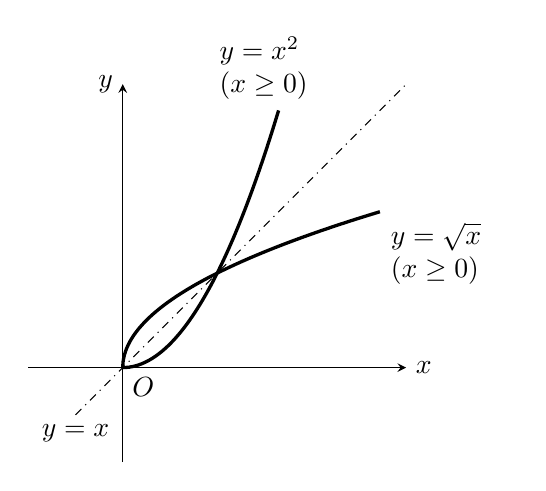
\begin{tikzpicture}[>=stealth, scale=1.2]
    \node[below right]{$O$};
\draw[->](-1,0)--(3,0)node[right]{$x$};
\draw[->](0,-1)--(0,3)node[left]{$y$};
\draw[dashdotted](-.5,-.5)node[below]{$y=x$}--(3,3);
\draw[domain=0:1.65, smooth, very thick]plot(\x, \x^2)node[above, text width=1.5cm]{$y=x^2$\\$(x\ge 0)$};
\draw[domain=0:1.65, smooth, very thick]plot(\x^2, \x)node[below right, text width=1.5cm]{$y=\sqrt{x}$\\ $(x\ge 0)$};


\end{tikzpicture}    
    \caption{}
\end{minipage}\hfill
\begin{minipage}{.45\textwidth}
    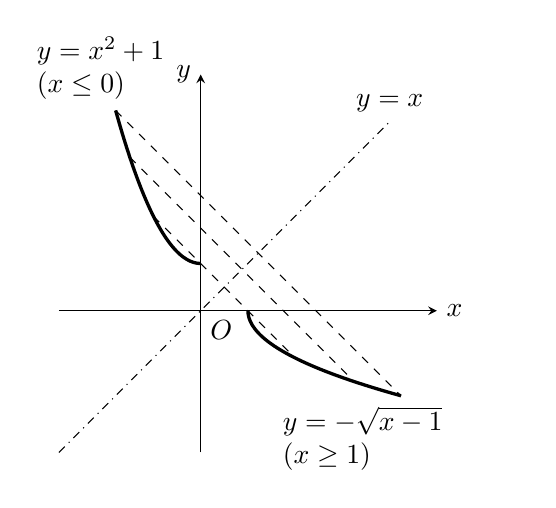
\begin{tikzpicture}[>=stealth, scale=.6]
    \node[below right]{$O$};
\draw[->](-3,0)--(5,0)node[right]{$x$};
\draw[->](0,-3)--(0,5)node[left]{$y$};
\draw[dashdotted](-3,-3)--(4,4)node[above]{$y=x$};
\draw[domain=0:-1.8, smooth, very thick]plot(\x, 1+\x*\x)node[above, text width=2cm]{$y=x^2+1$\\$(x\le 0)$};
\draw[domain=0:-1.8, smooth, very thick]plot(1+\x*\x, \x)node[below, text width=3cm]{$y=-\sqrt{x-1}$\\$(x\ge 1)$};
\draw[dashed](-1,2)--(2,-1);
\draw[dashed](-1.5,3.25)--(3.25,-1.5);
\draw[dashed](-1.8,4.24)--(4.24,-1.8);

\end{tikzpicture}  
    \caption{}    
\end{minipage}
\end{figure}

下面重点研究$f(x)$与$f^{-1}(x)$图象间的关系,从图2.30可以看出,函数$f(x)=x^2\; (x\ge 0)$和它的反函数$f^{-1}(x)=\sqrt{x}\; (x\ge 0)$的图象是以直线$y=x$为对称轴的对称图形(以后简称关于直线$y=x$对称)。从图2.31也可以看出,函数$f(x)=x^2+1\; (x\le 0)$和它的反函数$f^{-1}(x)=-\sqrt{x-1}\; (x\ge 1)$的图象关于直线$y=x$对称。

由此做出猜测:设$y=f(x),\; x\in A$的图象是$C$,它的反函数$y=f^{-1}(x),\; x\in B$的图象是$C'$,则$C$与$C'$关于直线$y=x$对称。欲证明这个猜测,须证明:
\begin{enumerate}[(1)]
    \item $C$上的每一个点关于$y=x$的对称点都在$C'$上;
\item $C'$上的每一个点关于$y=x$的对称点都在$C$上。
\end{enumerate}

\begin{proof}
\begin{enumerate}[(1)]
    \item 任取点$P(a,b)\in C\Longrightarrow b=f(a)\Longrightarrow a=f^{-1}(b)\Longrightarrow P'(b,a)\in C'$. $P(a,b)$与$P'(b,a)$的位置有什么关系?
\begin{enumerate}[(i)]
    \item 当$a=b$时,$P(a,b)$与$P'(b,a)$重合在直线$y=x$上.
    \item 当$a\ne b$时,我们来证明点$P$与点$P'$关于直线$y=x$对称。
    
    在$y=x$上任取一点$Q(c,c)$, 根据图2.32
\[\begin{split}
    |PQ|&=\sqrt{(a-c)^2+(b-c)^2}\\
    |P'Q|&=\sqrt{(b-c)^2+(a-c)^2}\\
\end{split}\]
$\therefore\quad |PQ|=|P'Q|$
\end{enumerate}

\begin{figure}[htp]
    \centering
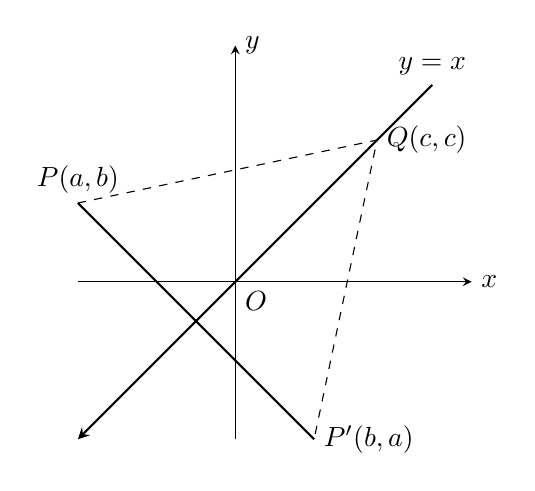
\begin{tikzpicture}[>=stealth]
\draw[->](-2,0)--(3,0)node[right]{$x$};
\draw[->](0,-2)--(0,3)node[right]{$y$};
\node[below right]{$O$};
\draw[->, thick](2.5,2.5)node[above]{$y=x$}--(-2,-2);
\draw[thick](-2,1)--(1,-2);
\draw[dashed](-2,1)node[above]{$P(a,b)$}--(1.8,1.8)node[right]{$Q(c,c)$}--(1,-2)node[right]{$P'(b,a)$};
\end{tikzpicture}
    \caption{}
\end{figure}


这说明$y=x$上任一点到$P$,$P'$的距离都相等,所以直线$y=x$是线段的垂直平分线。即点$P$与$P'$对称于直线$y=x$,即点$P$关于直线$y=x$的对称点在图象$C'$上。

由于点$P(a,b)$是在图象$C$上任取的,所以$C$上的每一个点关于$y=x$的对称点都在$C'$上。

\item 又由于$f^{-1}(x)$的反函数是$f(x)$,所以,$C'$上的每一个点关于$y=x$的对称点也必在$C$上.
\end{enumerate}

$\therefore\quad $图象$C$与$C'$关于直线$y=x$对称.
\end{proof}

\begin{example}
说明函数$f(x)=x^3+1$存在反函数的理由。求$f(x)$的反函数,画出反函数的图象。   
\end{example}

\begin{solution}
由于在$\R$上,$f(x)$单调增,从而确定$f(x)$的映射是从$\R$到$\R$上的一一映射,所以$f(x)$存在反函数$f^{-1}(x)$.
\[y=x^3+1\; (x\in\R)\Longrightarrow x=\sqrt[3]{y-1}\; (y\in\R)\]
因此:$y=\sqrt[3]{x-1}\; (x\in\R)$

$\therefore\quad f^{-1}(x)=\sqrt[2]{x-1}\; (x\in\R)$.

可利用熟知的$f(x)=x^3+1$的图象作关于直线$y=x$的对称图形而得出$f^{-1}(x)= \sqrt[2]{x-1}\; (x\in\R)$的图象(图2.33).
\end{solution}    

\begin{figure}[htp]
    \centering
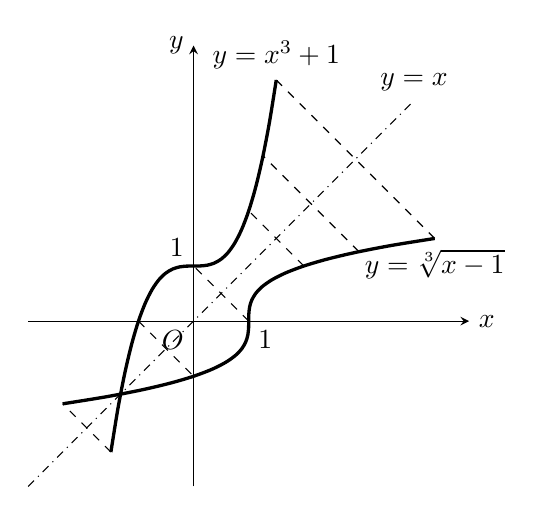
\begin{tikzpicture}[>=stealth, scale=.7]
\draw[->](-3,0)--(5,0)node[right]{$x$};
\draw[->](0,-3)--(0,5)node[left]{$y$};
\draw[domain=-1.5:1.5, smooth, very thick]plot(\x, 1+\x^3)node[above]{$y=x^3+1$};
\draw[domain=-1.5:1.5, smooth, very thick]plot(1+\x^3,\x)node[below]{$y=\sqrt[3]{x-1}$};
\node [below left]{$O$};
\draw[dashdotted](-3,-3)--(4,4)node[above]{$y=x$};
\node at (0,1)[above left]{1};
\node at (1,0)[below right]{1};
\draw[dashed](-1,0)--(0,-1);
\draw[dashed](-1.5,-2.375)--(-2.375,-1.5);
\draw[dashed](1,0)--(0,1);
\draw[dashed](2,1)--(1,2);
\draw[dashed](3,1.26)--(1.26,3);
\draw[dashed](4.375,1.5)--(1.5,4.375);



\end{tikzpicture}
    \caption{}
\end{figure}

\begin{example}
    求$f(x)=25-x^2\; (-5\le x\le 0)$
的值域。
\end{example}

\begin{solution}
\textbf{解法1:} $\because\quad $在$[-5,0]$上$f(x)$单调增.

$\therefore\quad f(-5)\le f(x)\le f(0)$即
\[\sqrt{25-25}\le f(x)\le \sqrt{25-0}\]
$\therefore\quad 0\le f(x)\le 5$.
即:$f(x)$的值域为$[0,5]$.

\textbf{解法2:}(利用反函数的定义域)

由$y=\sqrt{25-x^2}\; (-5\le x\le 0)\Longrightarrow x=-\sqrt{25-y^2}\; (y\ge 0)$

令$\begin{cases}
    25-y^2\ge 0\\
    y\ge 0
\end{cases}\Longrightarrow \begin{cases}
    y^2\le 25\\ y\ge 0
\end{cases}\Longrightarrow 0\le y\le 5$

$\therefore\quad f(x)$的值域是$[0,5]$.
\end{solution}


\section*{习题七}
\begin{center}
    \bfseries A
\end{center}

\begin{enumerate}
    \item 下列函数是否存在反函数?若存在,试求之:
\begin{enumerate}[(1)]
    \item $y=-2x-3\quad (x\in\R)$
    \item $y=x^5+1\quad (x\in\R)$
    \item $y=x^4\quad (x\le 0)$
    \item $y=\frac{-2}{x}\quad (x\in\R, \text{且}x\ne 0)$
    \item $y=-\frac{1}{x}+3\quad (x\in\R, \text{且}x\ne 0)$
    \item $y=\frac{x}{3x+5}\quad (x\in\R, \text{且}x\ne -\frac{5}{3})$
    \item $y=\frac{2x}{5x+1}\quad (x\in\R, \text{且}x\ne -\frac{1}{5})$
    \item $y=\sqrt{2x-4}\quad (x\ge 2)$.
\end{enumerate}

\item 已知$y=\sqrt{25-x^{2}}\quad (0\leq x\leq4)$, 它存在反函数吗?若存在,试求之。
\item 求下列函数的反函数。并写出原来函数及反函数的定义
域:
\begin{multicols}{2}
\begin{enumerate}[(1)]
    \item $y= \frac {1- x}{1+ x} $
    \item $y= 1- \sqrt{x- 2}$ 
\end{enumerate}
\end{multicols}
\end{enumerate}

\begin{center}
    \bfseries B
\end{center}
\begin{enumerate}\setcounter{enumi}{3}
    \item 下列函数的定义域怎样规定才有反函数?分别求出相应的
反函数(写出一种情况即可)。
\begin{multicols}{2}
\begin{enumerate}[(1)]
    \item $y= 3x^2- 1$ 
    \item $y= 2( x- 1) ^2+ 1 $
    \item $y= \sqrt{x^{2}- 4}$
    \item $y= \sqrt{9- x^{2}}$
\end{enumerate}
\end{multicols}
\item 求出$y=2|x|\quad (x<0)$的反函数,并在同一坐标系内画出两个函数的图象。
\item 求出函数$y=\frac{1}{x-1}\quad (x\ne 1)$的反函数,并在同一坐标系内画出两个函数的图象。
\item 求下列函数的值域:
\begin{multicols}{2}
\begin{enumerate}[(1)]
    \item $y=\frac{7}{x+2}\quad ( x\ne -2)$
    \item $y=\frac{x}{x+1}\quad (x\ne -1)$
    \item $y=\sqrt{16-x^2}\quad (0\le x\le 4)$
    \item $y=\sqrt{x^2-49}\quad (x\le -7)$
\end{enumerate}    
\end{multicols}
\end{enumerate}

\begin{center}
    \bfseries C
\end{center}

\begin{enumerate}\setcounter{enumi}{7}
    \item 已知函数$f(x)$在定义域上是单调增函数,求证它的反函数$f^{-1}(x)$也是单调增函数。
  \item   已知函数$f(x)$存在反函数$f^{-1}(x)$,且函数$f(x)$为奇函数,求证函数$f^{-1}(x)$也为奇函数。
\end{enumerate}

\section{复合函数}
我们在研究函数时常遇到下面的问题:

已知函数$f(x)=3x^2-5x+2$.
\begin{enumerate}[(1)]
\item 求$f(3)$、$f(-\sqrt{2})$、$f(a)$;
\item 若$u=x-1$,求$f(u)$。   
\end{enumerate}

\begin{analyze}
    $f(a)$表示$f(x)$在$x=a$处的值。欲求$f(a)$,只要在$f(x)$的表达式中以$a$代替$x$即可。
\end{analyze}

\begin{solution}
\begin{enumerate}[(1)]
    \item $f(3)=3\times 3^2-5\times 3+2=14$
\[\begin{split}
    f(\sqrt{2})&=3\left(\sqrt{2}\right)^2-5\times \sqrt{2}+2=8-5\sqrt{2}\\
    f(a)&=3a^2-5a+2\\
    f\left(\frac{1}{a}\right)&=3\times \left(\frac{1}{a}\right)^2-5\times \left(\frac{1}{a}\right)+2=\frac{3}{a^2}-\frac{5}{a}+2
\end{split}\]
\item $\because\quad u=x-1,\quad f(x)=3x^2-5x+2$

\[\begin{split}
    \therefore\quad f(u)&=3u^2-5u+2\\
    &=3(x-1)^2-5(x-1)+2\\
    &=3x^2-11x+10
\end{split}\]
\end{enumerate}
\end{solution}

\begin{rmk}
这里的$f(u)$实际上就是$f(x-1)$. 它是通过把$u=x-1$代入$y=f(u)$而构成的。像这样把$u=g(x)$代入$y=f(u)$而构造出来的函数$y=f[g(x)]$称为\textbf{复合函数}。
\end{rmk}

\begin{thm} {定义9}
   若函数$u=g(x)$,其定义域为$M$,值域为$N$,又有函数$y=f(u)$,它的定义域是$N$,这样就通过变量$u$构成了$x$的函数,记作$y=f[g(x)]$,则称$y$为$x$的复合函数,$u$叫做中间变量.
\end{thm}

\begin{example}
    已知$f(x)=2x^{2}+5x+7$, $g(x)=3x-2$, 
求$f[g(x)]$, $g[f(x)]$
\end{example}

\begin{analyze}
欲求$f[g(x)]$,只要以$g(x)$代换$f(x)$中的$x$,也就
是将$g(x)$的表达式填入下式中的括号内。
$$f[g(x)]=2(\quad)^{2}+5(\quad)+7$$    
\end{analyze}

\begin{solution}
\[\begin{split}
f[(g(x)]&=2(3x-2)^{2}+5(3x-2)+7\\
&=2\left(9x^{2}-12x+4\right)+5\left(3x-2\right)+7\\
&=18x^{2}-9x+5\\
g[f(x)]&=3(2x^{2}+5x+7)-2\\
&=6x^{2}+15x+19
\end{split}\]
\end{solution}

\begin{example}
\begin{enumerate}[(1)]
    \item  已知$f( x) = 3x+ 4$, $g( x) = \frac 1x$,求$g[f(x)]$的定义域.
    \item 若$f(x)$的定义域为$D=(0,3]$,求$f(x^2)$的定义域.
\end{enumerate}
  \end{example} 

\begin{solution}
\begin{enumerate}[(1)]
    \item $g[f(x)]=\frac{1}{f(x)}=\frac{1}{3x+4}$,欲使$g[f(x)]$有意义,须$3x+4\ne 0\Longleftrightarrow x\ne -\frac{4}{3}$
    
$\therefore\quad g[f(x)]$的定义域$D_1=\left(-\infty,-\frac{4}{3}\right)\cup\left(-\frac{4}{3},+\infty\right)$

\item $\because\quad f(x)$的定义域为$(0,3]$

$\therefore\quad 0<x^2\le 3 \Longleftrightarrow -\sqrt{3}\le x<0$ 或 $0<x\le \sqrt{3}$.

从而$f(x^2)$的定义域为$\left\{x\mid -\sqrt{3}\le x\le \sqrt{3},\; \text{且}\; x\ne 0\right\}$
\end{enumerate}
\end{solution}

\begin{example} 
    若$f(x-1)=2x^{2}-3x$, 求$f(x).$
\end{example}

\begin{solution}
\textbf{解法1:} (引入中间变量法)
设$u=x-1$, 则$x=u+1$, 代入原式,
$$f(u)=2(u+1)^{2}-3(u+1)=2u^{2}+u-1$$

$\therefore\quad f\left ( x\right ) = 2x^2+ x- 1$

\textbf{解法2:}(构造法,将原式右边构造成以$(x-1)$为“元”的解析式)
\[\begin{split}
    f(x-1)&=2x^{2}-3x=2(x-1)^{2}+4x-2-3x\\
    &=2\left(x-1\right)^{2}+\left(x-1\right)-1
\end{split}\]

$\therefore\quad f( x) = 2x^2+ x- 1$
\end{solution}

\section*{习题八}
\begin{center}
    \bfseries A
\end{center}

\begin{enumerate}
    \item 已知$f(x)=10x^2+1$, 求$f(x-1),\; f\left(\frac{x}{2}\right),\; f(x^{2}),\; f[f(x)]$
    \item 已知$f(x)=ax^2+bx+c$, 求证$f(x+3)-3f(x+2)+3f(x+1)-f(x)=0$
    \item 若$f(x)=2x-1$, $g(x)=x^{2}$, 求方程
$f[g(x)]=g[f(x)]$的根。
\end{enumerate}




\begin{center}
    \bfseries B
\end{center}

\begin{enumerate}\setcounter{enumi}{3}
    \item \begin{enumerate}[(1)]
    \item 若$f(x-1)=2x-5$, 求$f(x)$
    \item 若$f(x+1)=3x^2+10x+9, 求f(x)$
    \item 若$f\left(x+\frac1x\right)=x^2+\frac1{x^2}+1$, 求$f(x)$        
    \end{enumerate} 

 \item 若 $f(x-3)=x^{2}+2x+1$, 求$f(x+3)$
 \item 若$f\left(x-\frac1x\right)=x^2+\frac1{x^2}$, 求$f(x+1)+f(x-1)$
\end{enumerate}

\section{函数的值域}

对于给定的函数其值域也是确定的。准确而迅速地确定函数的值域对于研究函数的性质及运用函数的知识解决实际问题有重要的作用。下面介绍几种求函数值域的方法:

\subsection{利用已知函数的值域去求未知函数的值域}
例如:一次函数$y=kx+b\; (k\ne 0)$的值域是$y\in\R$;二次函数$y=x^2$的值域是$y\in [0,+\infty)$,反比例函数$y=\frac{k}{x}\; (x\ne 0)$的值域是$y\in (-\infty,0)\cup (0,+\infty)$,随着函数知识学习的深入,我们将掌握更多的具体函数的值域,为我们求函数值域的问题提供更多的依据。

\begin{example}
求函数$y=x^{2}-4x-5$的值域.    
\end{example}

\begin{solution}
    $y=(x-2)^{2}-9$

$\because\quad (x-2^{2})\ge 0\qquad \therefore\quad (x-2)^{2}-9\ge -9$

$\therefore\quad y\in[-9,+\infty)$
\end{solution}

\begin{example}
   求函数$y=5-\sqrt{-x^{2}+2x+3}$的值域。 
\end{example}

\begin{solution}
    $y=5-\sqrt{4-(x-1)^{2}}$

    $\because\quad 4-(x-1)^{2}\ge 0\qquad \therefore\quad x\in[-1,3]$

    $\because\quad  x\in[-1,3]\qquad \therefore\quad (x-1)^{2}\in [0,4]$

$\therefore\quad 4-(x-1)^{2}\in[0,4]$

$\therefore\quad\sqrt{4-(x-1)^{2}}\in[0,2]$

$\therefore\quad 5-\sqrt{4-(x-1)^{2}}\in[3,5]$.

$\therefore\quad $函数的值域为$y\in[3,5]$.
\end{solution}

\begin{example}
    求函数$y=x+\sqrt{1-2x}$的值域.
\end{example}

\begin{solution}
设$t=\sqrt{1-2x}\ge 0$, 则$x=\frac{1-t^2}{2}$

$\therefore\quad y=\frac{1-t^2}{2}+t=-\frac{1}{2}(t-1)^2+1$

$\because\quad $当$t\ge 0$时,$-\frac{1}{2}(t-1)^2\le 0$

$\therefore\quad y=-\frac{1}{2}(t-1)^2+1\le 1$

即函数$y=x+\sqrt{1-2x}$的值域为$(-\infty,1]$
\end{solution}

由本例可以看出利用换元法可以把未知函数的值域问题转化为已知的二次函数值域问题来解决,但是应注意换元后所得新函数的定义域对函数值域的影响。

\subsection{利用函数的单调性求函数的值域}
\begin{example}
    求函数$y=x^2-4x+5,\quad x\in [3,5]$的值域。
\end{example}

\begin{solution}
    在定义域$x\in[3,5]$上函数$y=x^2-4x+5$是单调增函数,
    
$\therefore\quad $当$x=3$时,取得函数最小值2;当$x=5$时,取得函数最大值10。

$\therefore\quad $函数的值域为$y\in [3,5]$
\end{solution}


\subsection{利用反函数的定义域来求函数的值域}
\begin{example}
    求函数$y=\frac{4x+5}{3x-2}$的值域。
\end{example}

\begin{solution}
由所给的函数反解出$x$,得:$x=\frac{2y+5}{3y-4}$,使其有意义的$y$值为
\[y\in \left(-\infty,\frac{4}{3}\right)\cup \left(\frac{4}{3},+\infty\right)\]
即为所求函数的值域.

\end{solution}

\begin{example}
    求函数$y=\frac{x^2+3x-4}{2x^2-5x+3}$的值域。
\end{example}

\begin{solution}
原函数可化简为 $y=\frac{x+4}{2x-3}\quad (x\ne 1)$

反解出$x=\frac{3y+4}{2y-1}$,使其有意义的$y$值为$y\in\R$且$y\ne\frac{1}{2}$.

又$\because\quad x\ne 1$

$\therefore\quad \frac{3y+4}{2y-1}\ne 1$, 即$y\ne 5$.

$\therefore\quad $所求函数的值域为$y\in(-\infty,-5)\cup\left(-5,\frac{1}{2}\right)\cup \left(\frac{1}{2},+\infty\right)$
\end{solution}

\subsection{利用判别式法求函数的值域}

\begin{example}
 求函数
$y=\frac{2x}{x^2-4x+3}$的值域。   
\end{example}

\begin{solution}
    去分母整理成关于$x$的二次型得
\[yx^2-(4y+2)x+3y=0\]
当$y\ne 0$时,上式是关于$x$的二次方程

$\because\quad x\in\R$

$\therefore\quad y$的允许值可由判别式确定,即
\[\Delta =(4y+2)^2-12y^2\ge 0\]
整理得$y^2+4y+1\ge 0$, 
解之得$y\le -2-\sqrt{3}$或$y\ge -2+\sqrt{3}$且$y\ne 0$.

当$y=0$时,方程为$-2x=0$,解之得$x=0$,
即当$x=0$时,$y=0$,

$\therefore\quad y=0$也是函数的函数值。

$\therefore\quad $所求函数的值域为
$y\in (-\infty,-2-\sqrt{3}]\cup [-2+\sqrt{3},+\infty)$
\end{solution}

\section*{习题九}
\begin{center}
    \bfseries B
\end{center}

求下列函数的值域:
\begin{multicols}{2}
    \begin{enumerate}
    \item $y=x^2+4x,\quad (x\in[-5,-3])$
    \item $y=\frac{1}{x-2},\quad \left(x\in\left[0,\frac{3}{2}\right]\right)$
    \item $y=5-2x+\frac{4}{x+1},\quad (x\in[1,3])$
    \item $y=3+2\sqrt{x^2+2x+5}$
    \item $y=3-\sqrt{8+2x-x^2}$
    \item $y=\frac{5-2x}{x-3}$
    \item $y=\frac{x^2+x-6}{x^2-3x+2}$
    \item $y=2x-3+\sqrt{13-4x}$
    \item $y=\frac{4}{x^2-2x-15}$
    \item $y=\frac{(2x+5)(x+1)}{x}$
\end{enumerate}
\end{multicols}

\section{本章小结}
\subsection{知识结构分析}
\subsubsection{映射与函数的逻辑关系}

\begin{center}
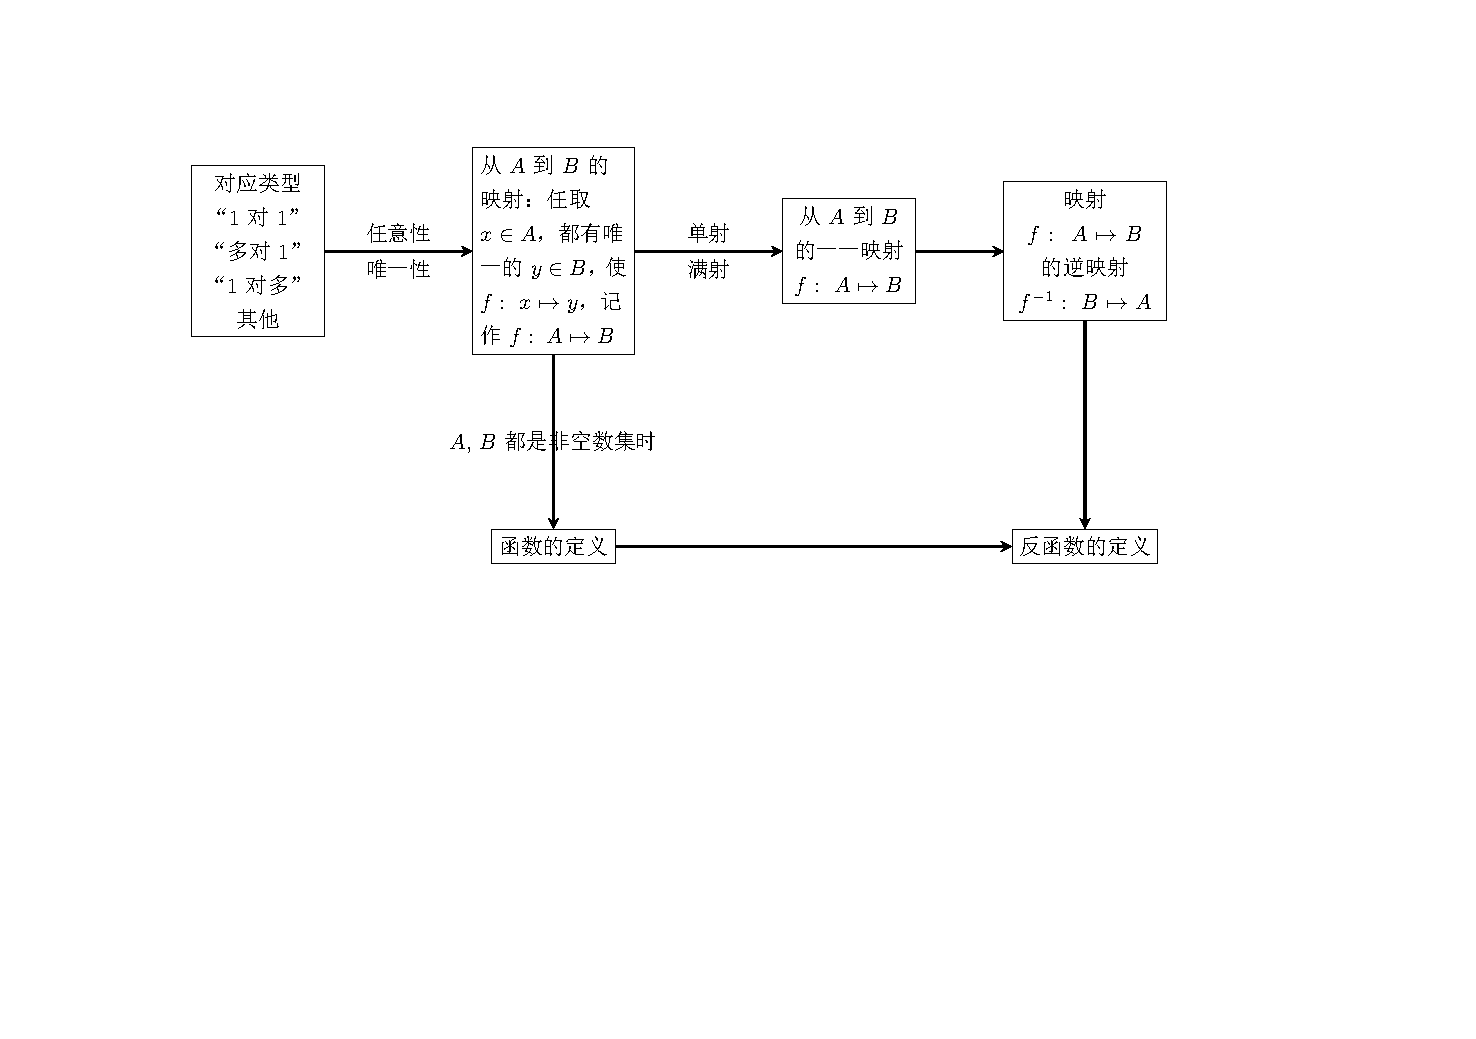
\includegraphics[scale=.75]{fig/fig2.pdf}
\end{center}

应注意:
\begin{enumerate}
    \item 每个定义都要正确叙述;
    \item 箭头指示了概念间的逻辑关系,应从理论发展的脉络上去理解。
\end{enumerate}

\subsubsection{函数概论的知识结构}

\begin{tikzpicture}[>=stealth]
\node[draw, rectangle](A) at (1,3+.75)[text width=1.5cm, align=center] {复合函数}; 
\node[draw, rectangle](B) at (1,0.75)[text width=1.5cm, align=center] {函数的\\定义}; 
\node[draw, rectangle](C) at (1,-3+.75)[text width=1.5cm, align=center] {函数\\表示法}; 
\draw[->, very thick](B)--(A);
\draw[->, very thick](B)--(C);

\node (E1) at (4,6)[right]{定义域(求法:归结为解不等式组)};
\node (E2) at (4,4.5)[right]{值域$\Bigg\{$};
\node (E21) at (5.25,5)[right]{值域的定义、求法};
\node (E22) at (5.25,4.5)[right]{特殊值(最大值、最小值)的求法};
\node (E23) at (5.25,4)[right]{给函数值的范围,求自变量的取值范围};
\node (E3) at (4,2.75)[right]{增减性$\Big\{$};
\node (E31) at (5.5,3)[right]{单调函数的定义、实质及判断};
\node (E32) at (5.5,2.5)[right]{单调区间的求法};
\node (E4) at (4,1.25)[right]{奇偶性$\Big\{$};
\node (E41) at (5.5,1.5)[right]{奇(偶)函数的定义、实质及判断};
\node (E42) at (5.5,1)[right]{奇偶性的应用};

\node (E5) at (4,.25)[right]{周期性(三角中待学)};

\node (E6) at (4,-1)[right]{画法$\Big\{$};
\node (E7) at (4,-2.5)[right]{看图认性质:函数性质与图象的一致性};
\node (E61) at (5.25,-.75)[right]{先讨论函数性质};
\node (E62) at (5.25,-1.25)[right]{再用描点法画图$\Big\{$};

\node (E71) at (8.5,-1)[right]{体现性质};
\node (E72) at (8.5,-1.5)[right]{标记特殊点};

\draw[decorate, very thick, decoration={brace, amplitude=10pt}](4,.25)--node[left=10pt]{性质}(4,6);

\draw[decorate, very thick, decoration={brace, amplitude=5pt}](4,-2.5)--node[left=7pt]{图象}(4,-1);

\draw[decorate, decoration={brace, amplitude=10pt}, very thick](2.5,-1.75)--(2.5,3);
\end{tikzpicture}

(这些内容的复习要结合有关小节进行)

\subsubsection{应掌握以下几点}
反函数存在的充要条件,反函数的求法,从函数的有关性质预测其反函数的性质(见2.6节)。


\subsubsection{图象的几种几何变换}
\begin{enumerate}
    \item $y=f(x)\longrightarrow y=f(x)+c$
   \hfill (纵向平移:上移$c$个单位)
    \item $y=f(x)\longrightarrow y=f(x+m)$
    \hfill   (横向平移:左移$m$个单位)
    \item $y=f(x)\longrightarrow y=-f(x)$
    \hfill   (关于$x$轴的对称变换)
    \item $y=f(x)\longrightarrow y=f(-x)$
    \hfill    (关于$y$轴的对称变换)
    \item $y=f(x)\longrightarrow y=|f(x)|$
    \item $y=f(x)\longrightarrow y=f(|x|)$
\end{enumerate}

\subsection{本章应着重掌握的数学思想}
\begin{enumerate}
\item 映射的思想:$\map{f}{A}{B},\quad \map{f}{x}{y},\; x\in A$.
\item 函数的思想:$y=f(x),\quad x\in A$.
\item 数、形结合的思想。
\item 函数、方程、不等式互相转化的思想。
\end{enumerate}

\section*{复习题二}
\begin{center}
    \bfseries A
\end{center}

\begin{enumerate}
    \item 设$M=\left\{a,b\right\}$, $N=\left\{x,y\right\}$, 从$M$到$N$的映射可以构造\blank
种,请用图示法表示这些映射。
\item 已知映射$\map{f}{A}{B}$, 其中$A=\{(x,y)\mid x\in \R,\; y\in \R\}$, 
$B=\{(\overline{x},\overline{y})\mid \overline{x}=x+y,\; \overline{y}=xy,\; x,y\in\R\}$,
$\map{f}{(x,y)}{(\overline{x},\overline{y})}$, $(x,y)\in A$, 则$(8,15)$的原象是\blank.

\item (选择题)使对应法则$\map{f}{x}{y}=x^2$成为从$X$到$Y$上的一
一映射的条件是(\quad ).
\begin{multicols}{2}
\begin{enumerate}[(A)]
    \item $X=Y=\R$
    \item $X=R,\; Y=\{\text{非负实数}\}$
    \item $X=\{\text{非负实数}\},\; Y=\R$
    \item $X=Y=\{\text{非负实数}\}$
\end{enumerate}
\end{multicols}

\item (选择题)$f( x) = \sqrt{x^{2}- 5x- 6}$ 的定义域是$F$, $g(x)=\sqrt{x-6}\cdot\sqrt{x+1}$ 的定义域是$G$, 则$F$ 与$G$ 的关系是(\quad).
\begin{multicols}{4}
    \begin{enumerate}[(A)]
        \item $F=G$
        \item $F\subset G$
        \item $F\supset G$
        \item $F\cap G=\emptyset$
    \end{enumerate}
    \end{multicols}
\item (选择题) 已知$0<a<1$, 设$x=a,\; y=2a,\;z=a^2$, 则$x,y,z$的大小关系是(\quad)
\begin{multicols}{4}
    \begin{enumerate}[(A)]
        \item $x<y<z$
        \item $z<y<x$
        \item $z<x<y$
        \item $x<z<y$
    \end{enumerate}
    \end{multicols}
\end{enumerate}

\begin{center}
    \bfseries B
\end{center}

\begin{enumerate}\setcounter{enumi}{5}
    \item (选择题)$f(x)=ax^2-6ax+1\; (a>0)$,则下列关系中正确的是(\quad)
\begin{multicols}{2}
    \begin{enumerate}[(A)]
        \item $f(\sqrt{2})>f(\sqrt{3})$
        \item $f\left(\frac{\pi}{2}\right)>f(\pi)$
        \item $f(\sqrt{5})<f(3)$
        \item $f(-1)<f(1)$
    \end{enumerate}
    \end{multicols}
\item (选择题)$f(x)=ax^3+cx+5$,已知$f(-3)=-3$,则$f(3)$等于(\quad)
\begin{multicols}{4}
    \begin{enumerate}[(A)]
        \item 3
        \item $-3$
        \item 2
        \item 13
    \end{enumerate}
    \end{multicols}
\item $f(x)$是偶函数,$g(x)$是奇函数,且$f(x)+g(x)=\frac1{x-1}$,
求$f(x)$与$g(x)$的表达式。

\item $f(x)=x^{3}+bx^{2}+cx$是奇函数,$g(x)=x^{2}-(c-2)x+5$是偶函数,则$b=\blank$, $c=\blank$.

\item 奇函数$F(x)$, 当$x<0$时,$F(x)=f(x)$, 则$F(x)$的完整表达式是\blank.

\item $y= \frac{1}{2} x+ a$与$y=3-bx$互为反函数,则$a=\blank$, $b=\blank$.
    
\item (选择题)$y=ax+b$与它的反函数是同一函数,则下列(\quad )中的数据是正确的。
\begin{multicols}{2}
    \begin{enumerate}[(A)]
        \item $a=1,\; b=0$
        \item $a=-1,\; b=0$
        \item $a=\pm 1,\; b=0$
        \item $a=1,\; b=0$;或$a=-1,\; b\in\R$
    \end{enumerate}
    \end{multicols}

\item (选择题)在函数$y= x- 1$, $y= x+ 1$,  $y= 2x- 1$, $y=2x+1$, $y=x^{2}$, $y=\sqrt{x}$, $y=x^{3}$, $y=\sqrt[{3}]{x}$中互为反
函数的有(\quad)
\begin{multicols}{4}
    \begin{enumerate}[(A)]
        \item 1对
        \item 2对
        \item 3对
        \item 4对
    \end{enumerate}
    \end{multicols}

\item $f(x)=\frac{x+1}{x-1}$, 则$f^{-1}(\sqrt{2})=\blank$.

\item $f(x)=3x-5$,则$f^{-1}[f(x)]=\blank$.

\item 将函数$y=\frac{1}{x}$的图象经过平移可以画出$y=\frac{x+3}{x+2}$的图
象,平移的步骤是\blank, \blank.
\end{enumerate}

\begin{center}
    \bfseries C
\end{center}

\begin{enumerate}\setcounter{enumi}{16}
\item 证明$f(x)=\frac x{x^2+1}$在$(-1,1)$上是增函数。

\item  函数$y=(x-1)^3+1$的图象的中心对称点的坐标是什么? 
\item 若$A=\{x\mid 10-3x-x^{2}\ge 0\}$, $B=\{x\mid m+1\leq x\leq 2m+1\}$, 
求实数$m$, 使$A\cap B\neq\emptyset$.
\item 奇函数$f(x)$在定义域$(-1,1)$上是单调 递增的,且
$f\left(1-a\right)+f\left(1-a^2\right)<0$, 求$a$的取值范围。
\end{enumerate}














